\documentclass{sig-alternate}
%\documentclass{acm_proc_article-sp}

\usepackage{graphicx}
\usepackage{url}
\usepackage[noend]{algpseudocode}
\usepackage{algorithmicx,algorithm}
\usepackage{listings}
\usepackage{paralist}
\usepackage[skip=0pt]{subcaption}
%\usepackage[tight]{subfigure}
\usepackage{eepic}
\usepackage{xcolor}

\newcommand\addtypes[1]{%
  \lstset{morekeywords=[3]{#1}}}

\newtheorem{definition}{Definition}
\newtheorem{theorem}{Theorem}
\newtheorem{lemma}[theorem]{Lemma}

\newcommand{\remove}[1]{}
\newcommand{\full}[1]{}
\newcommand{\short}[1]{#1}
\newcommand{\eshcar}[1]{\noindent{\textcolor{violet}{\{{\bf eshcar:} \em #1\}}}}
%%%%%%%%%%pseudo code
\newcommand{\const}[1]{\textsc{#1}}
\newcommand{\tuple}[1]{\ensuremath{\left\langle {#1} \right\rangle}}

\newcommand{\medserver}{\ensuremath{\mathcal{TSO}}}
\newcommand{\dbserver}{\ensuremath{\mathcal{DB}}}
\newcommand{\logger}{\ensuremath{\mathcal{LOG}}}

\begin{document}
%
% --- Author Metadata here ---
\permission{Permission to make digital or hard copies of all or part of
this work for personal or classroom use is granted without fee provided 
that copies are not made or distributed for profit or commercial advantage 
and that copies bear this notice and the full citation on the first page. 
Copyrights for components of this work owned by others than the author(s) 
must be honored. Abstracting with credit is permitted. To copy otherwise, 
or republish, to post on servers or to redistribute to lists, requires 
prior specific permission and/or a fee. Request permissions from 
Permissions@acm.org.}
\conferenceinfo{SYSTOR '14}{June 10-12 2014, Haifa, Israel}
\CopyrightYear{2014} % Allows default copyright year (20XX) to be over-ridden -
% IF NEED BE.
\crdata{978-1-4503-2920-0/14/06\\ DOI 10.1145/2611354.2611366}  %
% Allows default copyright data (0-89791-88-6/97/05) to be over-ridden - IF NEED BE.
% --- End of Author Metadata ---

\title{Reconciling Transactional and Non-Transactional Operations in Distributed Key-Value Stores}
%


\numberofauthors{3} %  in this sample file, there are a *total*
% of EIGHT authors. SIX appear on the 'first-page' (for formatting
% reasons) and the remaining two appear in the \additionalauthors section.
%
\author{
%
% 1st. author
\alignauthor
Edward Bortnikov\\
       \affaddr{Yahoo Labs}\\
       \affaddr{Haifa, Israel}\\
       \email{ebortnik@yahoo-inc.com}
% 2nd. author
\alignauthor
Eshcar Hillel\\
       \affaddr{Yahoo Labs}\\
       \affaddr{Haifa, Israel}\\
       \email{eshcar@yahoo-inc.com}
% 3rd. author
\alignauthor 
Artyom Sharov\titlenote{Research done while interning with Yahoo Labs, Haifa.}\\
       \affaddr{Technion, CS}\\
       \affaddr{Haifa, Israel}\\
       \email{sharov@cs.technion.ac.il}
}

\date{30 July 1999}
% Just remember to make sure that the TOTAL number of authors
% is the number that will appear on the first page PLUS the
% number that will appear in the \additionalauthors section.

\maketitle
\begin{abstract}

NoSQL databases were initially designed to provide extreme scalability and
availability for Internet applications, often at the expense of data consistency. The recent generation
of Web-scale databases fills this gap, by offering transaction support. However, transaction
processing implies a significant performance overhead on online applications
that only require atomic reads and writes. The state-of-the-art solutions are either static separation 
of the data accessed by transaction-enabled and native applications, or complete 
``transactification'' of the latter, which are both inadequate. 

We present a scalable transaction processor, {\em Mediator}, that enjoys the best of 
both worlds. It preserves the latencies of atomic reads and writes, without compromising 
data safety. We introduce a lightweight synchronization protocol that enables conflict 
resolution between transactions and native operations that share data in a distributed
database. We evaluate Mediator's implementation on top of the HBase key-value store 
on a large-scale testbed, and show that it substantially outperforms 
the traditional approach on a vast majority of mixed workloads.
In particular, Mediator achieves a significantly larger throughput for all 
workloads in which the fraction of native operations exceeds $50\%$.

%despite a slight overhead incurred to the transactional traffic, 
\end{abstract}

% A category with the (minimum) three required fields
%\category{H.4}{Information Systems Applications}{Miscellaneous}
%A category including the fourth, optional field follows...
%\category{D.2.8}{Software Engineering}{Metrics}[complexity measures,
% performance measures]

\category{H.2.4}{Database Management}{Systems}[Transaction processing,
Distributed databases] 
\terms{Algorithms, Reliability, Performance}
%\keywords{search engine caching, real-time indexing}

\hyphenation{No-SQL}
\hyphenation{da-ta-ba-ses}
\hyphenation{ser-vers}
\hyphenation{pa-ra-mount}

\section{Introduction}
\label{sec:intro}

% Scale, scale, scale
Modern Internet applications employ data stores that scale to the entire population 
of online users. For example, personalized content recommendation services  require 
maintaining profiles for hundreds of millions of unique users. Traditional SQL data 
management systems cannot scale up with these requirements, leading to a new generation 
of not-only-SQL, or NoSQL, databases -- e.g., Google's Bigtable~\cite{BigTable2006}, Apache Hadoop HBase\footnote{\small{\url{http://hbase.apache.org/}}}, etc. These technologies have been designed 
for extreme simplicity (key-value store API), scalability (data partitioning across thousands of machines), 
and reliability (redundant storage). In parallel, the proliferation of affordable high-end hardware 
(multi-core CPU's, inexpensive RAM, SSD storage) enabled building NoSQL databases capable of serving 
data at memory speeds~\cite{Corfu2012,RAMCloud2011,FDPlus2012}.

% Transactions are great
Historically, NoSQL databases only allowed atomic reads and writes of individual items. 
More recent systems (e.g., Google's Percolator~\cite{Percolator2010} and HBase's 
Omid\footnote{\small{\url{https://github.com/yahoo/omid}}}~\cite{Omid2014})
introduce transaction processing~\cite{GrayTP1993} for complex applications that
require ACID semantics while accessing multiple items. NoSQL transaction processors
implement consistency models extensively studied by the database community~\cite{Papadimitriou1979, FeketeTODS2005}.
They have been shown to scale well with the database size. 

% We have a problem
Transaction processing does not come for free. Every transaction incurs latency penalties at its begin 
and commit boundaries. In throughput-oriented applications that perform long
transactions latency is not of big concern, and indeed the overhead is minor~\cite{Omid2014}. 
However, it is well-pronounced in online, interactive settings, which are
the main focus of this work.
The faster the underlying database is, the larger the toll. Table~\ref{tab:latencies} exemplifies the impact of ``transactifying'' HBase 
reads and writes by Omid in a high-speed environment (fully evaluated in
Section~\ref{sec:eval}).
Latencies start growing as every operation is framed as a transaction (column
2).
They double as part of the traffic is batched in short and long transactions
(columns 3 and 4, respectively).

%\setlength{\belowcaptionskip}{0pt}
\setlength{\abovecaptionskip}{3pt}
\begin{table} [t]
\centering{
\begin{tabular}{ccccc}
%& {\bf \small{Native}} & {\bf \small{Transactified}} & {\bf
%\small{Transactified} }    & {\bf \small{Transactified} } \\
& {\bf native} & {\bf trans} & {\bf
trans }    & {\bf trans } \\
%&                    &                              & {\bf short transactions}
% & {\bf medium-size transactions} \\
&                    &        {\bf + none }         & {\bf + short
} & {\bf + long } \\
%&                    &                              & {\bf in the background} &
% {\bf in the background} \\
\hline
{\bf Read}  & 3.9 & 5.2 & 6.0 & 9.2 \\
{\bf Write}  & 8.3 & 9.5 & 10.3 & 14.0  \\
\end{tabular}
}
\caption{\bf{\small{The impact of transactification
(\emph{trans}) on HBase \emph{native} operations latencies (ms).
Transaction processing adds a surplus that grows with the length of transactions
executed in the background (\emph{none}, \emph{short}, \emph{long}).
}}}
\label{tab:latencies}
\end{table}

% Why this is nontrivial
We would like to avoid automatically converting the atomic database operations
into transactions. Unfortunately, running them side by side with transactional traffic on shared data 
without any coordination is error-prone. Consider, for example, an imaginary social application, 
in which user statuses can be either directly posted by the users, or speculated by the system, 
based on a variety of signals (status history, location, time of day, sensor data, friends' posts,  etc.). 
In the latter case, the system updates the status unless the user has recently
posted a new one.
Therefore, it performs a transaction that (1) reads the user's status, and possibly some other data, 
(2) does some computation, and (3) writes the status back. In contrast, a human-originated status 
update is blind -- it must complete in the real time, and needs not be transactional. In a %na\"{\i}ve 
non-coordinated implementation, the transaction is not aware of this update,
and may overwrite it with a stale speculated value.
%, so the update is \emph{lost}.

An additional problem with the non-coordinated design is exposure to uncommitted data.
The transaction processing layer prevents transactions from reading each other
intermediate modifications that may eventually roll-back~\cite{GrayTP1993}.
However, in a heterogeneous environment, native reads can retrieve transaction's
\emph{dirty} writes.

% Goal and challenge
Our goal is to preserve the original performance of native operations while
maintaining the familiar consistency guarantees for them as well as for
transactions. This challenge is amplified in distributed databases, in which the data is partitioned among 
multiple servers. In this context, any solution must take care not to impede
the datapath scalability, by introducing minimum synchronization.     

We present {\em Mediator} --- Mixed Database Access Transaction Oracle --- 
a scalable transaction processor that %allows to benefit from both worlds. 
guarantees data consistency in the presence of native operations. To the best 
of our knowledge, this problem has not been addressed by the database community before. 
%The contributions of our work are as follows.

%Theoretical model
\remove{We establish a formal definition of the consistency model for systems
supporting transactions and native operations, and prove Mediator's compliance
with it.}
We establish a consistency model for systems
supporting transactions and native operations. Namely, we extend the popular
{\em serializability\/}~\cite{Papadimitriou1979} and {\em snapshot isolation\/} (SI)~\cite{FeketeTODS2005} models to accommodate 
the native traffic semantics. The extension is not straightforward since native operations 
are not captured as transactions, and the consistency requirements are relaxed for them. 
The formal definition of the models and Mediator's correctness proofs are
deferred to the full version of this paper~\cite{full}.

%Distributed Algorithm
%We present an algorithm that satisfies the required safety properties.
Similarly to earlier work~\cite{WeikumTIS2001,Omid2014}, 
Mediator exploits multi-version concurrency control at the database layer 
to implement its consistency model. The unique challenge is installing 
a logical order between transactions, which are ordered by a centralized logical 
clock, and native operations, accessing multiple independent 
servers. We introduce \emph{temporal fencing\/} -- a novel protocol that
loosely synchronizes the servers' local clocks with the global clock. 
The algorithm trades performance optimization of native operations 
for an extra overhead imposed on transactions. 

We implement a working prototype of Mediator on top of HBase, and extensively evaluate it 
on a distributed testbed. We study Mediator's performance tradeoffs by comparing
it to an Omid-powered system that automatically converts native operations into transactions. The results 
emphasize the performance impact incurred to native traffic by Omid.
More importantly, we show that Mediator's {\em overall\/} system performance is superior 
for a vast majority of the considered mixed traffic patterns. In particular, its throughput 
is higher for all workloads that contain at least $50\%$ native operations. 
%Therefore, a slight overhead incurred to the transactional traffic is justified 
%by preserving the native traffic's performance. 
%The bulkier the transactional traffic is, the more advantageous our system becomes. 

The rest of this paper is structured as follows. Section~\ref{sec:overview} sketches Mediator's system architecture. 
Section~\ref{sec:semantics}  
informally presents mixed traffic semantics, and 
Section~\ref{sec:algorithm} describes the algorithms implementing two
consistency models.
Section~\ref{sec:eval} depicts and analyzes the evaluation results. 
%Rigorous model definition and correctness proofs appear in
% Section~\ref{sec:correctness}.
Finally, we survey related work in Section~\ref{sec:related}, 
and conclude with Section~\ref{sec:conc}.

\section{System Overview}
\label{sec:overview}

\hyphenation{com-mit-ted}

% Distributed DB
Mediator operates on top of a distributed key-value store with a
{\em get\/}/{\em put\/} API that provides a read/write access to data items identified by unique keys. For scalability, 
the data can be partitioned over multiple nodes. In this context, all accesses 
to a given item are served by a single node ({\em database server}). The get/put
API is called {\em native}, in contrast with Mediator's API that is {\em transactional}. The database
serves both types of traffic. Native clients are unaware of concurrent transactions. 

Mediator assumes 
multi-version concurrency control~\cite{GrayTP1993} in the underlying database.
Namely, every update creates a new version of the data item, and multiple versions 
can be accessed in parallel. The transaction processor maintains a global logical clock 
to timestamp all transactional writes. The execution is optimistic -- i.e., each transaction
runs unobstructed until commit, whereupon consistency is enforced. At that point, 
semantic conflicts are detected through version timestamps, and the compromised 
transactions are aborted. 

Mediator shares many design principles with Omid~\cite{Omid2014}. Similarly to
Omid, Mediator employs a  standalone {\em transaction status oracle} service (TSO), which maintains the clock and tracks the state required for guaranteeing the safety
properties.  Transactional clients use this context to read the correct data versions 
and to timestamp their writes. A transaction communicates with the TSO twice -- upon begin, 
to retrieve the required state, and upon commit, to resolve the conflicts with the concurrent 
transactions. The key for scalability is keeping the TSO separate from the datapath.

% TSO scalability
The TSO is highly optimized, to prevent it from becoming the system's bottleneck. 
A transaction starts getting tracked only once it issues a commit request. A client
communicates to the oracle the set of keys accessed by the transaction.
The Mediator TSO stores it in a compressed Bloom filter~\cite{Bloom1970} form,
hence each transaction's footprint is fixed and small.  Mediator adopts Omid's 
optimization of replicating the oracle's state to the client upon transaction begin,
to enable local decision-making~\cite{Omid2014}. For clients with persistent TSO 
connections, this replication is incremental and efficient.

\remove{
% Clock propagation
Guaranteeing a logical order between transactions and native operations 
requires some coordination of the local database server clocks with the global clock. 
For this, Mediator clients piggyback the global clock's value retrieved from the TSO 
on top of the datapath requests served by the database (Section~\ref{sec:algorithm}). 
The oracle does not communicate with the database directly, to avoid becoming a bottleneck. 
}
% Deferred updates 
%In rare cases when transactions get aborted, their changes are rolled back. 
In multi-version databases, concurrent transactions are protected 
from reading non-committed writes by creating new versions with timestamps
that are beyond the read horizon. This approach is non-applicable 
in our setting, since native reads that simply retrieve the latest data versions 
must be protected. Instead, Mediator clients buffer the updates locally, and write them 
back upon commit. Prior to updating the database, the client atomically appends its 
modification set to the write-ahead log (WAL).
This is in contrast to other transaction processor
implementations~\cite{Percolator2010,Omid2014} writing eagerly to the database.
These implementations exploit the durability of database updates and therefore
avoid managing a separate log.
Mediator's performance for the {\em transactional\/} 
part of the traffic is therefore a-priori inferior to eager-write systems. 
Section~\ref{sec:algorithm} describes the optimizations that target this gap.

% Recovery
Since Mediator's writes are deferred until commit, it never needs to roll back aborted 
transactions. However, a failure of either a client or a database server in the middle 
of a distributed write-back can leave transactions--that are committed in the
log--incomplete.
While the algorithm guarantees that subsequent transactions always observe 
a consistent database state, some of them might get blocked and eventually
abort due to dependencies on incomplete transactions. To guarantee progress, 
the TSO helps uncompleted transactions finish their database update. It
periodically initiates a helper process that locates their commit records in the log, and replays 
them in an idempotent way~\cite{GrayTP1993}. Transactions that failed to log their
changes prior to the helper's execution are 
%cut off by setting a low watermark on 
%the commit timestamp. Hence, they effectively 
(possibly spuriously) aborted. 

\begin{figure}

\centering {
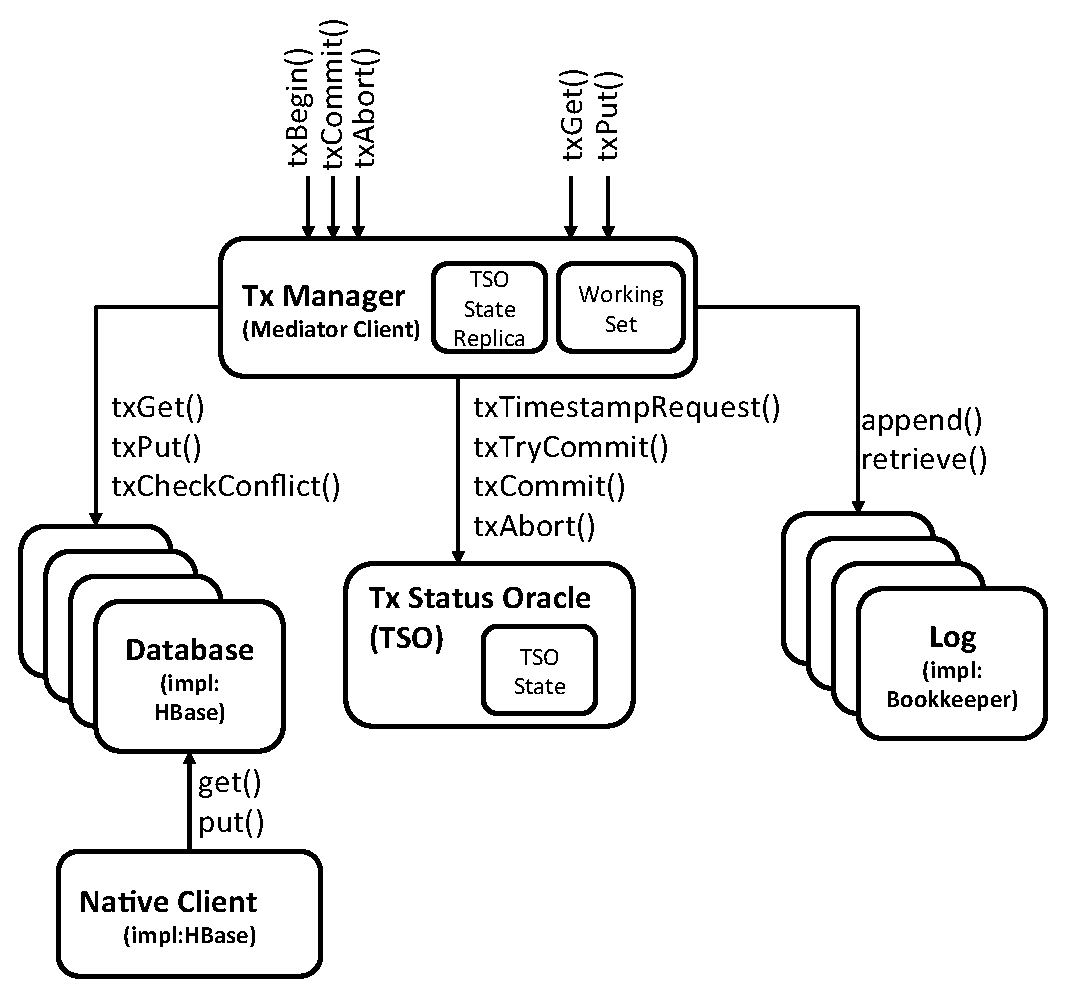
\includegraphics[width=3in,clip]{Figs/mediator_arch.eps}
}

\caption{\bf{\small{Mediator architecture. The transaction manager (Mediator client)
employs three backend services -- the database, the log, and the transaction status oracle (TSO). 
The database serves native clients directly, and provides Mediator clients with a backdoor API. 
}}}
\label{fig:mediator_arch}
\end{figure}
 
Oracle's failures are handled similarly. Upon recovery, the TSO replays the log, 
and aborts all transactions that initiated a commit before the crash but
failed to log their changes.
Hence, the volatile state that the TSO has maintained for them prior to the
failure needs not to be restored.  Before becoming operational, the TSO sets its
clock sufficiently ahead of the committed transactions and the local clocks of all live database servers,
to guarantee correctness. Obviously, until the recovery completes, 
no transactions can commit, however, native operations execute regularly. 
The rest of the paper focuses on non-failure scenarios. 

Figure~\ref{fig:mediator_arch} depicts Mediator's architecture, and highlights
the component API's.
We implement Mediator on top of two open source products -- a multi-versioned key-value store (HBase) and a shared log service
 (Bookkeeper\footnote{\footnotesize{\url{http://zookeeper.apache.org/bookkeeper/}}}~\cite{Bookkeeper2013}).
Both scale horizontally across multiple machines. 
%The algorithm requires minor changes at the HBase server side. 





\section{Mixed Traffic Semantics}
\label{sec:semantics}

In classical (transaction-only) implementations the
versions of an item are ordered according to the temporal sequence of the
transactions that created these versions. Informally, in serializable systems all
transactions appear to execute sequentially. The weaker model of snapshot isolation decouples the consistency of the gets and the puts of a transaction.
That is, all reads within a transaction see a consistent view of the
database, as though the transaction operates on a private snapshot of the
database taken before its first read. 
In addition, concurrent transactions are not allowed to modify the same data.
This 
%In the classical (transaction-only) implementation of SI, the disjoint writes
% property
ensures that among two transactions that produced a version of an
item, one commits before the other starts.  

Mixed-traffic implementations need to consider how
to pin native operations within this order.
%==================
A straightforward semantic for mixed traffic captures native
operations as single operation transactions. This surely guarantees no
updates are lost and no reads are dirty.
However, it may introduce unnecessary overhead on native operations.
% and results in inefficient implementations.


The detour we suggest from converting native operations to transactions is
twofold.
Similar to traditional NoSQL, (i)~native operations cannot abort, and 
(ii)~no guarantees are provided
on the order of native gets in the serialization (with respect 
to each other). 
That is, a process that sequentially retrieves two different items being 
updated in parallel by some transaction might observe an older version in the 
second read. 

%================

We revisit our web application example to demonstrate the main
theoretical challenges of such systems.
A backend transaction \emph{tx} reads the status $s_0$ of a user, computes a refined status $s_2$ and tries to
update the user's status record. It should succeed (commit) only if the user is
not writing a new status $s_1$ at the same time. Furthermore, should the user write
a new status before \emph{tx} commits, no friend of the user (applying a
transaction or native operations) should see status $s_2$.

Figure~\ref{fig:mixedaccess} depicts an execution of this scenario. 
Assume the initial timestamps of all items are $0$. 
Transaction {\em tx\/} starts (at $t_0$), reads item $z$ (the user status) and
returns $s_0$, writes $s_2$ to $z$, and finally commits.
The user entry is
updated with $s_2$ only after the transaction is guaranteed to commit
(otherwise it might be visible to the user's friends).
While \emph{tx} is committing, after it is logged as committed 
and just before it writes the new value to $z$ (with timestamp $t_1$), a
concurrent native put, \emph{op}, by the user writes a new status $s_1$ to $z$.

Due to data partitioning, there is no single point of decision, and the
timestamps assigned to \emph{op} is determined by the data server
accomodating the item (the user record).
A possible na\"{\i}ve approach is to associate \emph{op} with the item's
previous timestamp plus some increment.
This is, however, insufficient for correctness. For example, if \emph{op} is
assigned %The na\"{\i}ve approach associate this native operation 
with an arbitrary (positive) timestamp $t$, $t<t_1$, a friend of the user
reading the status after the transaction completes sees status $s_2$ and $s_1$
is ``lost''. 

%\setlength{\belowcaptionskip}{6pt}
\begin{figure}
        \centering
        \begin{subfigure}[b]{0.5\textwidth}
                %\flushleft
                \centering
                \scalebox{0.80}{\input{Figs/mixedaccess.eepic}}
                \caption{If \emph{tx} commits but \emph{op}'s timestamp is
                $t<t_1$, then \emph{op} is ``lost''.}
                \label{fig:mixedaccess}
        \end{subfigure}%
         %add desired spacing between images, e. g. ~, \quad, \qquad etc. 
          %(or a blank line to force the subfigure onto a new line)
         
        \begin{subfigure}[b]{0.5\textwidth}
                \centering
                \scalebox{0.80}{\input{Figs/temporalfence.eepic}}
                \caption{Temporal fences (depicted as dashed lines) guard safety
                by aborting \emph{tx}.}
                \label{fig:temporalfence}
        \end{subfigure}
          
        \begin{subfigure}[b]{0.5\textwidth}
                \centering
                \scalebox{0.80}{\input{Figs/disjoint.eepic}}
                \caption{Temporal fences guard safety by serializing \emph{op}
                after \emph{tx}.}
                \label{fig:disjoint}
        \end{subfigure}
        \caption{\bf{\small{Execution example: transaction $tx$
        (process $C_1$) versus a native put $op$ (process
        $C_2$).}}}\label{fig:mixed}
\end{figure}

It is also desirable to avoid trivial solutions ``separating'' native
operations and transactions in time. That is, to assign \emph{op} with a 
small timestamp $t$, $t \ll t_0$ such that it is ``lost in the past'', or a very
big timestamp $t \gg t_1$ such that it is ``lost in the future'' and never read
by any transaction. To enforce this restriction, the semantics require the
serialization of all accesses of transactional and non-transactional operations to the same
item by the same process to be in the same order as executed by the process. 
This property is denoted \emph{per-process item order}.

To conclude, mixed traffic semantics (1)~require transactions to satisfy some
consistency model, be it serializability, snapshot isolation or any other
model, (2)~require native operations not to abort and (3)~require
operations to satisfy the per-process item order. The formal extension of the
classical serializability and snapshot isolation models for mixed traffic
appear in the full version of this paper.

\section{Mediator Algorithm}
\label{sec:algorithm}

Mediator's way to satisfy these semantics---\emph{temporal fences},
effectively partitions the logical timing of native puts into epochs framed by transaction begin and
commit operations.  
%
We present the algorithm focusing on SI
consistency; Section~\ref{sec:ser} elaborates on the adjustments 
required to support serializability.  In what follows, \emph{write set} refers
to data items written by a transaction and \emph{read set} to items it reads. 
A \emph{read-write} transaction performs both get and put operations,
a \emph{read-only} transaction performs only get operations (its write set is
 empty), and a \emph{write-only} transaction performs only put operations (its
 read set is empty). A \emph{put} transaction is a write-only transaction
 writing to a single item.


\subsection{Temporal Fences}
\label{sec:temporal fences}

To accommodate mixed traffic, Mediator embeds 
a standard centralized transaction manager, with an original mechanism to pin 
the versions produced by native puts in the total order without compromising
the transactions safety. %Due to data partitioning, there is no single point of
% decision, and
Native writes are stamped by each data server independently, whereas
transactional writes inherit the timestamps issued centrally by the TSO.
Combining the two mechanisms---one centralized and the other
distributed---requires care.

Each database server maintains a local clock.  
This clock is used to stamp native puts, which in turn increase it in increments 
of $\delta$. Each transaction is associated with two values of the global TSO
clock.
Transaction's reads are associated with its
start timestamp, and writes with its commit
timestamp.
Upon each database access, the transaction synchronizes the local clock with
one of these values--i.e., the server's clock is promoted to be (at
least) this value. This value then serves as a fence -- no subsequent native
operation to this server is assigned with timestamp lower than the fence. Specifically,
the $\delta$ increment defer the timing of subsequent native put
operations to this server beyond the fence value. 
The global clock assigning transactional timestamps grows by $\Delta$ upon each 
timestamp request. 
To avoid the trivial time-separation solution we set $\Delta \gg \delta$. This
ensures native puts that are executed within the 
epoch marked by two temporal fences, are serialized within this epoch.

In the execution example, when {\em tx\/} accesses the data server 
for the first time, it assigns its local clock to be $t_0$ (first fence),
thereby guaranteeing that $op$'s timestamp is greater than $t_0$, and it is not
lost in the past.
%hence the snapshot property
% holds.
Prior to writing a new value to $z$, {\em tx\/} verifies no
concurrent put (specifically, a native one) has written to $z$. %and to log the
% transaction for recovery purposes.
Upon this conflict testing, {\em tx\/} promotes the local clock to $t_1$, $t_1
\geq t_0 + \Delta$ (second fence).
Therefore, the write conflict validation is safe; the set of native writes
between $t_0$ and $t_1$ is sealed. 
In the scenario depicted in Figure~\ref{fig:temporalfence}, 
\emph{op} is assigned with timestamp $t$, $t_0 + \delta = t < t_1$, 
{\em tx\/} identifies the conflict and aborts. In the scenario depicted in
Figure~\ref{fig:disjoint}, \emph{op}'s timestamp is $t_1 + \delta=t$, hence
there is no conflict and \emph{tx} commits.
As $\delta \ll \Delta$ \emph{op} is not lost in the future, and is visible to
subsequent transactions.
%A later transaction
%by $C_2$ starts at least at timestamp $t_2 \geq t_1+\Delta > t_1 + \delta $ and
%the per-process item order is guaranteed as well.

With this in mind, Mediator's algorithm is simple and intuitive.
The begin timestamp of a transaction
%which serves as a read timestamp and 
is
a temporal fence. A get returns the latest version of the item prior to this timestamp.
Write accesses to the data server by transactions are deferred to commit,
and a put simply privately records the key-value pair. Upon commit of read-only
transactions, no further action is required
since the snapshot property holds: a {\em no-commit\/} optimization. 
A put transaction commits locally, 
by applying a native put thereby avoiding the commit
overhead: a \emph{local-commit} optimization.

Other transactions apply a \emph{two-phase commit}.
\full{Figure~\ref{fig:txn_diagram} visualizes the protocol. }
The first phase (conflict testing) consists of a centralized part and a distributed 
part. The former generates a commit timestamp 
and tests for inter-transaction conflicts. The latter installs the commit timestamp 
as a temporal fence at the data servers accommodating the write set, and
performs the transaction-vs-native conflict test. The second phase (write-back) logs the new values 
for durability, and ultimately stores them in the database, making the changes 
visible to other transactions and native operations.

%
\remove{
\begin{figure}
\centering {
\includegraphics[width=3.2in, clip]{Figs/txn_diagram.epsi}
}
%\vskip .1in
\caption{\bf{\small{Success scenario of \emph{tx} from Figure~\ref{fig:mixed}. \emph{sync} installs temporal fences to the database.}}}
\label{fig:txn_diagram}
%\vskip -.2in
\end{figure}
%
}

\full{
\setlength{\abovecaptionskip}{0pt}
\begin{figure}
%\centering 
%\includegraphics[width=3.2in, clip]{Figs/commitseq.eps}
\begin{minipage}{0.72\textwidth}
%\centerline{
\includegraphics[width=0.72\textwidth, clip]{Figs/txseq.eps}
%}
\end{minipage}
\caption{\bf{\small{Example: transaction success path. Temporal fences are installed upon {\em sync\/} calls.}}}
\label{fig:txn_diagram}
\end{figure}
\setlength{\abovecaptionskip}{10pt}
}

Next, we describe the implementation details, including 
the pseudo-code.
The code is structured in a way that can be easily adapted to support 
serializability.% (Section~\ref{sec:ser}).
%Our model assumes that each operation is an atomic step, whereas this is not
%always the case in the algorithm we suggest. To be able to prove the
% correctness of the algorithm, 
%The description of each non-atomic operation includes a
%reference to its {\em linearization point\/} -- an atomic event upon which 
%the operation is considered as executed. The order of these linearization
% points essentially defines the execution. 
% for lack of space, the proofs are deffered to the full version of the paper.

\subsection{Transaction Manager Implementation}
\label{sec:si:client}

The key parts of Mediator's API implementation appear in Algorithm~\ref{alg:client}. 
For simplicity, we assume that (1) a transaction reads and writes any item 
at most once, and (2) if a transaction writes an item, it does not read it
afterwards\footnote{These assumptions are not restrictive -- modeling these
(redundant) operations is possible but obscures the presentation.}. 

%Mediator's client is a transaction manager that invokes
%the database, the TSO, and the logger. 
%In this context, the database 
%de-multiplexes the batch operations among the data servers hosting the affected
% keys, in accordance with some partitioning scheme. The latter perform the requests atomically 
%and independently.

%Mediator keeps track of the transactions it has initiated. 
A transaction 
is represented by a descriptor\full{(Algorithm~\ref{alg:client}}, which holds the start and commit timestamps, 
as well as the write set (set of key-value-timestamp tuples). The latter is 
used to identify conflicts upon commit. 
The implementation supporting serializability also needs to maintain the read
set.

A transaction begins by retrieving a unique start timestamp from the 
TSO\full{, which is used to initialize the transaction's descriptor and further serves as
its handle.}\short{.} Similar to Omid~\cite{Omid2014}, the incremental
changes of the status oracle's state are piggybacked on the response to facilitate local decisions. 

A transactional get ($\const{txGet}$) reads from the database the latest value 
preceding the start timestamp.\full{ (line~\ref{line:getlast})}
%The asynchronous nature of write-back by other transactions can cause a read 
%to retrieve a version that is not the latest.
%a value written by a transaction that committed 
%immediately before but has not made its modifications durable yet. 
The timestamp of the expected version is registered in the local 
replica of the TSO's state\full{ (line~\ref{line:islatest})}, however the value
itself might not be stored in the data server yet. A failure to retrieve the
correct version triggers a sequence of attempts to re-read this version\full{
(line~\ref{line:retryget})}, and ultimately an abort in case they all fail\full{ (line~\ref{line:abortget})}.
%The point where the value is added to the transaction read set is the
% linearization point of the get operation.

\remove{
It verifies, using the local replica of $\medserver$ state, that indeed no later transaction committed a new version (line~\ref{line:islatest}). 
If the transaction reads the latest version, the timestamped value is 
%added to the read set (line~\ref{line:addread}), and 
returned to the application (line~\ref{line:retval}). Otherwise, the version 
is not yet available in the database due to asynchronous write-back, and should
be re-read (line~\ref{line:retryget}). If multiple reads fail to retrieve the expected version, the transaction eventually aborts (line~\ref{line:abortget}).
}

\begin{algorithm} [t]
\small
\caption{\small Mediator API implementation - \full{begin, put, get, commit and
abort}\short{get and commit} (snapshot isolation)} 
\label{alg:client} 

\full{
\begin{lstlisting}[mathescape]
struct KeyValVersion {
  Key $key$
  Val $val$
  Timestamp $ts$
}
class Transaction {
  Timestamp $ts_s$ // start timestamp
  Timestamp $ts_c$ // commit timestamp
  Set$\tuple{KeyValVersion}$ $writeSet$
  Set$\tuple{KeyValVersion}$ $readSet$
}
\end{lstlisting}
}
\begin{algorithmic}[1]
\makeatletter\setcounter{ALG@line}{0}\makeatother

\full{
\Function{txBegin}{} 
	\State $ts \gets $ \medserver.txTimestampRequest() \label{line:startts}
	\Statex \Comment{piggyback: sync \medserver\ state replica}
	\State initTx($ts$) \label{line:inittx}
	\State \Return $ts$	\label{line:retts} \Comment{timestamp as unique id}
\EndFunction
\vspace{7pt}
}
\Function{txGet}{Timestamp $ts$, Key $key$}
	\State $tx \gets$ getTx($ts$) 
	\For{\const{retry\_get} times} \label{line:retryget}
	  \State $\tuple{val,ts_{val}} \gets$ \dbserver.txGet($key$,$ts$) \label{line:getlast}
	  %\Statex 
	  \Comment{sync \dbserver\ with $ts$} 
	  \If{$ts_{val} \geq$ latestCommitted($key$,$ts$)} \label{line:islatest}
	  	\Statex \Comment{latest timestamp before $ts$ in the \medserver\ state replica}
	  	\State $tx$.addToReadSet($key$,$val$,$ts_{val}$) \label{line:addread}
	  	\State \Return $val$ \label{line:retval}
	  \EndIf
	\EndFor
	\State txAbort($ts$) \label{line:abortnotlatest}\Comment{unable to read latest value} \label{line:abortget}
\EndFunction
\vspace{7pt}
\full{
\Function{txPut}{Timestamp $ts$, Key $key$, Val $val$}
	\State $tx \gets$ getTx($ts$) 
	\State $tx$.addToWriteSet($key$,$val$,$ts$) \label{line:addwrite}
\EndFunction
\vspace{7pt}
}
\Function{txCommit}{Timestamp $ts$}
	\State $tx \gets$ getTx($ts$) 
	\If{readOnly($tx$)}
		\State \Return \Comment{committed successfully} \label{line:readonly}
	\EndIf
	\If{singleWriteOnly($tx$)}
		\State $\tuple{key,val,ts} \gets$ $tx$.writeSet.first()
		\State \dbserver.put($key$, $val$) \Comment{local write} \label{line:localupdate}
		\State \Return \Comment{committed successfully}
	\EndIf
	\State $ok \gets$ tryCommit($ts$, \const{ww}) \label{line:trycommit}
	\If{$ok$}
		\State writeVals($tx$) \label{line:writevals}
	\EndIf
\EndFunction
\vspace{7pt}
\full{
\Function{txAbort}{Timestamp $ts$}
	\State removeTx($ts$) \label{line:removeabort} \Comment{notify the invoking application}
\EndFunction
\vspace{7pt}
}
\Function{tryCommit}{Timestamp $ts$, ConflictType $type$}
	\State $tx \gets$ getTx($ts$) 
	\Statex \Comment{check txs conflicts against \medserver}
	\State $tx.ts_{c} \gets $ \medserver.txTryCommit($tx$,$type$) \label{line:checktso}
	\If{$tx.ts_{c} = \bot$}
		\State txAbort($ts$) \label{line:aborttso}
		\State \Return \const{false} \label{line:negtso}
	\EndIf
	\Statex \Comment{check natives conflicts against \dbserver}
%	\State $ok \gets$ checkNativeConflict($tx$, $type$) \label{line:checkdb}
	\If{$type$ = \const{ww}} 
		\State $confSet \gets $ $tx$.writeSet \Comment{\const{ww} conflicts} \label{line:dbwritekeys} 
	\EndIf
	\If{$type$ = \const{rw}} 
		\State $confSet \gets $ $tx$.readSet \Comment{\const{rw} conflicts} \label{line:dbreadkeys}
	\EndIf 
%	\Statex \Comment{check conflicts against \dbserver\ and sync it with $ts_{c}$}
	\State $ok \gets$ \dbserver.txCheckConflict($confSet$, $tx.ts_{c}$) \label{line:checknat}
	\If{$!ok$}
		\State txAbort($ts$) \label{line:abortdb}
	 	\State \medserver.txAbort($tx$) \label{line:abort}
		\State \Return \const{false} \label{line:negdb}
	\EndIf
	\State \Return \const{true} \label{line:trycommitok}
\EndFunction
\vspace{7pt}
\remove{
\Function{checkNativeConflict}{Transaction $tx$, ConflictType $type$} 
	\If{$type$ = \const{ww}} 
		\State $confSet \gets $ $tx$.writeSet \Comment{\const{ww} conflicts} \label{line:dbwritekeys} 
	\EndIf
	\If{$type$ = \const{rw}} 
		\State $confSet \gets $ $tx$.readSet \Comment{\const{rw} conflicts} \label{line:dbreadkeys}
	\EndIf 
	\Statex \Comment{check conflicts against \dbserver\ and sync it with $ts_{c}$}
	\State \Return \dbserver.txCheckConflict($confSet$, $tx.ts_{c}$) \label{line:checknat}
\EndFunction
\vspace{7pt}
}
\Function{writeVals}{Transaction $tx$}
	\State \logger.append($tx$.writeSet) \Comment{write ahead logging} \label{line:wal}
	\State \dbserver.txPut($tx$.writeSet, $ts_{c}$) \Comment{batch write} \label{line:batch}
	\State \medserver.txCommit($tx$) \label{line:commit}
\EndFunction

\end{algorithmic}
\end{algorithm}

A transactional put\full{ (\const{txPut})} adds the key-value pair to the write
set stamped with the start timestamp\full{ (line~\ref{line:addwrite})}.
%(linearization point).
This timestamp is used to check for conflicts upon commit.

Upon commit (\const{txCommit}) of a read-only transaction no further action
is required%
%Hence, these transactions are immediately committed 
%without calling $\medserver$ 
\full{ (line~\ref{line:readonly})}. %, and this is the linearization point.
A put transaction commits locally, by performing the respective native put
operation\full{ (line~\ref{line:localupdate})}.

Other transactions \full{follow the sequence depicted in
Figure~\ref{fig:txn_diagram}. It }invoke \const{txTryCommit} at the TSO and
\const{txCheckConflict} at the database, to verify transaction-vs-transaction
and transaction-vs-native conflicts, respectively (first phase of the two-phase
commit).
Note that the SI implementation checks for write-write ($\const{ww}$) conflicts.
Then (second phase), the transaction dumps its write set\full{
(line~\ref{line:writevals})} to the log\full{ (line~\ref{line:wal})} and to the database\full{
(line~\ref{line:batch})}.
\full{Upon completion, the client notifies the TSO, to enable the server-side 
bookkeeping\full{ (line~\ref{line:commit})}.}
%The linearization point of a commit
%operation of these transactions requires some care. If the transaction is
%durable, i.e., executed line~\ref{line:wal}, then the linearization point  is
%the step where the transaction appended its the commit timestamp to the ring
%(line~\ref{line:append}). Otherwise, it is not considered as executed yet.


\subsection{Transaction Status Oracle Implementation}
\label{sec:si:server}

The TSO %provides a set of operations specified in Section~\ref{sec:overview}. 
%All its API's are atomic. %ensures transaction atomicity and isolation via manipulation of
maintains  an ordered circular buffer (\emph{ring}) of transaction entries. %\footnote{
%\footnotesize{This data structure is mainly inspired by the \emph{RingSTM} algorithm for software transactional %memory~\cite{Spear2008}.}}.
%(see Section~\ref{sec:related} for more details).
The ring's entries describe only transactions that invoked 
\const{txTryCommit}, saving space and redundant processing.
A transaction commits by enqueuing an entry into the ring, therefore its
 position in the ring is its explicit serialization with respect to other 
transactions.  

The TSO's data structures appear in  Algorithm~\ref{alg:medserver}. A ring entry 
holds the transaction's commit timestamp, its status, and the write set's keys 
encoded as Bloom filters~\cite{Bloom1970} for compactness. The status is initially 
\const{active}, indicating that the transaction is serialized 
with respect to other transactions, but still has to check conflicts with native 
puts and write to the database. Upon a commit or abort notification,
the status is updated accordingly. Bloom filters help to efficiently 
test set membership -- in particular, compute the intersection between
transaction write sets to detect conflicts. The flip side of using them is
manifested in false intersections, which yield spurious aborts.

\remove{
%It uses a \emph{ring} structure to capture the serialization of the transactions, with respect to each other; it does not capture the order of native operations with respect to the transactions.
 Each entry in the ring describes an updating transaction and consists of four fields: commit timestamp (\emph{$ts_c$}), a Bloom filter representing the write set (\emph{writeBF}), a set of keys, either the write set or read set keys, depending on the consistency model (\emph{keySet}), and a \emph{status} field. 
Due to memory limitations, old entries are collected from the ring; \emph{$ts_{min}$} stores the minimum timestamp from which the ring maintains transactional history.

A ring entry initializes \emph{writeBF} and \emph{keySet} (lines~\ref{line:writebf} and~\ref{line:writekeys}). 
The \emph{status} of an entry in the ring is initially \const{active} (line~\ref{line:active}) indicating that the transaction is serialized with respect to other transactions, but it has to check conflicts with native operations and to update the database with its writes. When the transaction commits or aborts, the \emph{status} is set to \const{committed}% (line~\ref{line:committed})
, or \const{aborted}% (line~\ref{line:aborted})
, respectively (the pseudo-code of these methods is omitted).
}

\begin{algorithm} [t]
\small
\caption{\small \medserver\ methods (snapshot isolation)} \label{alg:medserver}
\begin{lstlisting}[mathescape]
struct TxEntry {
  Timestamp $ts_c$
  Status $status$ // 	$\left\{\const{active},\const{committed},\const{aborted}\right\}$
  BloomFilter $writeBF$
}
class Ring {
  Timestamp $ts_{min}$ // earliest timestamp
  TxEntry $head$
  TxEntry $tail$
}
\end{lstlisting}

\begin{algorithmic}[1]
\makeatletter\setcounter{ALG@line}{50}\makeatother
\full{
\Function{txTimpstampRequest}{} \Comment{atomic}
	\State \Return getNextTimestamp() \label{line:currts}\Comment{add $\Delta$}
\EndFunction
\vspace{7pt}
}
\remove{
\Function{txCommit}{Transaction $tx$}
	\State $entry \gets $ getEntry($tx.ts_{c}$)
	\State $entry.status \gets$ \const{committed} \label{line:committed}
\EndFunction
\vspace{7pt}
\Function{txAbort}{Transaction $tx$}
	\State $entry \gets $ getEntry($tx.ts_{c}$)
	\State $entry.status \gets$ \const{aborted} \label{line:aborted}
\EndFunction
\vspace{7pt}
}

\Function{txTryCommit}{Transaction $tx$, ConflictType $type$}
	\If{$ts_{min} > tx.ts_{s}$} \label{line:lessthanmin}
		\State \Return $\bot$ \Comment{too long a tx - abort} \label{line:tsonotok}
	\EndIf
	\State $writeKeys \gets $ getKeys($tx$.writeSet) \label{line:writeset}
%	\State $readKeys \gets $ getKeys($tx$.readSet) \label{line:readset}
	\State $new \gets $ initTxEntry($writeKeys$)
	\If{$type$ = \const{ww}} 
		\State $confSet \gets $ $tx$.writeSet  \Comment{\const{ww} conflicts} \label{line:tsowritekeys}
	\EndIf
	\If{$type$ = \const{rw}} 
		\State $confSet \gets $ $tx$.readSet \Comment{\const{rw} conflicts} \label{line:tsoreadkeys}
	\EndIf 
\label{line:confkeys}
	\State $ts \gets $ checkAndAppend($confSet$, $new$) \label{line:append}
	\State \Return $ts$ \Comment{timestamp or $\bot$}
\EndFunction

%\end{algorithmic}
%\end{algorithm}


%\begin{algorithm} \caption{Auxilliary methods for checking conflicts} \label{alg:aux}
%\begin{algorithmic}[1]
%\makeatletter\setcounter{ALG@line}{70}\makeatother
%\Statex \Comment{Mediator client methods}

%\Statex \Comment{\medserver\ methods}
\full{
\vspace{7pt}
\Function{initTxEntry}{Set$\tuple{Key}$ writes} 
	\Statex \Comment{allocates new entry}
	\State $new.writeBF \gets$ getBloomFilter(writes) \label{line:writebf}
%	\State $new.keySet \gets$ checkList \label{line:writekeys}
	\State $new.status \gets$ \const{active} \label{line:active}
	\State \Return $new$
\EndFunction
}
\vspace{7pt}
\Function{checkAndAppend}{Set$\tuple{KeyValVersion}$ confSet, TxEntry new}
	%\Statex 
	\Comment{atomic}
%	\State $lastVisited \gets $ getFirst()
%	\For{\const{retry\_commit} times}
%		\State $last \gets $ getLast()
		\State $new.ts_{c} \gets $ getNextTimestamp() \Comment{add $\Delta$} \label{line:committs}
%		\For{$current = last \to lastVisited$}
		\For{current $= tail \to head$} \label{line:tailtohead}
			\For{$item \in confSet$}
				\Statex \Comment{check conflict with concurrent txs}
				\If{$current.ts_{c} < item.ts$} \label{line:notconc}
					break
				\EndIf
				\If{current.status $\neq$ \const{aborted}} \label{line:tsocheckconf}
					\If{isMember(item, current.writeBF)} \label{line:intersect}
						\State \Return $\bot$ \Comment{conflict - abort} \label{line:appendnotok}
					\EndIf
				\EndIf
			\EndFor
		\EndFor
%		\State addLast($new$,$last$) \Comment{append after last}
		\State append($new$,$tail$) \label{line:appendentry}\Comment{append to tail} \label{line:appendtail}
%		\If{$!ok$}
%			\State $lastVisited \gets $ last
%			\State continue \Comment{try again} 
%		\EndIf 
		\State \Return $new.ts_{c}$ \Comment{serialization succeeded} \label{line:appendok}
%	\EndFor	
%	\State \Return $\bot$ \Comment{failed too many times - abort}
\EndFunction
%\vspace{10pt}
%\Function{checkConf}{TxEntry new, TxEntry entry} 
%	\If{entry.status $\neq$ \const{aborted}} \label{line:tsocheckconf}
%		\If{intersect(new.keySet,entry.writeBF)} \label{line:intersect}						%			\State \Return \const{false} \Comment{conflict - not ok}
%		\EndIf
%	\EndIf
%	\State \Return \const{true} \Comment{no conflict - ok}
%\EndFunction
%\vspace{10pt}
%\Function{intersect}{TxEntry new, TxEntry entry} 
%	\Statex\Comment{check for WW conflicts}
%	\State \Return intersect(new.writeBF,entry.writeBF)
%\EndFunction

\end{algorithmic}
\end{algorithm}

\const{txTryCommit\/} detects inter-transaction conflicts. A transaction
acquires a commit timestamp\full{ (line~\ref{line:committs})},
and traverses the ring from tail to head\full{ (line~\ref{line:tailtohead})}
validating the write set with the preceding non-aborted transactions\full{
(lines~\ref{line:notconc}-\ref{line:intersect})}.
%(The lookup in the list of active transactions in undecided state is omitted for brevity.)
%check is approximate, since the past transactions' write sets are captured by Bloom filters. 
%Since the ring is ordered by commit time, the check stops when it encounters a transaction that has committed before the new one started (line~\ref{line:notconc}). 
Finally, a new entry is appended to the ring\full{ (line~\ref{line:appendtail})},
and the commit timestamp is returned\full{ (line~\ref{line:appendok})}.
Long-running transactions that started before $ts_{min}$--the minimum timestamp
from which the ring maintains transactional history--abort\full{
(line~\ref{line:tsonotok})}.

The ring is periodically garbage-collected -- complete transaction entries that do not 
overlap with active transactions are deleted. Transactions for which no completion 
notification has been received remain in the ring until their final status is discovered 
by the helper process that runs periodically in the background
(discussed in Section~\ref{sec:overview}).

The algorithm's correctness
%(Lemmas~\ref{lemma:singleput},~\ref{lemma:si}) 
depends on the assumption
that native put timestamps never exceed the next transaction timestamp.  
For all practical purposes, this is achieved by setting $\Delta \gg \delta$ 
(e.g., $\Delta=2^{20}$ and $\delta=1$ for a $64$-bit value clock). 
To maintain the invariant, even when no transactional traffic arrives for a
very long time, the TSO periodically increments the global clock by
$\Delta$.
\remove{
In addition, the clocks can theoretically wrap around (which is highly unlikely with 64-bit values). 
A slight modification of the local clock's update code (omitted for clarity) can 
identify and handle this problem. 
\eshcar{should we say this if we don't elaborate how?}
}

%Upon the TSO's recovery, the local and global clocks must be re-synchronized. To achieve this, the oracle runs a special no-op transaction to collect all the local clock values, and sets the global clock beyond them.

%eshcar: removed appologies
%The TSO's scalability can be boosted by partitioning it across multiple
% machines, such that transaction entries are stored at different nodes. The only shared part
%is the global clock, which can be implemented very
% efficiently~\cite{Corfu2012}.
%In this setting, the transaction-vs-transaction conflict resolution requires a 
%agreement among multiple TSO servers. Although each individual server handles
% all commit requests, the per-request overhead is scaled down. We leave this optimization 
%to future work. 

\subsection{Database Support}
\label{sec:si:database}

\remove{
This section presents the changes to the database server code to support mixed traffic access.
%The main novelty we introduce here is a simple structure capturing the timestamp that is assigned to native put and get operations. 
Their core is a new policy for managing the server's logical clock. 
The latter is synchronized with the global clock upon transactional accesses, 
and is locally incremented upon native puts. 
%Recall that the timestamp-based API is deprecated for external native operation usage, however we use it internally as part of our adaptations.
}

The database code adjustments for Mediator are modest. They summarize to 
a new policy for managing the server's local clock. Local clocks synchronize 
with the global clock upon transactional accesses, and incremented upon 
native puts. Algorithm~\ref{alg:db} depicts the implementation.

A native get simply retrieves the latest version of the data item. 
A native put atomically increments the clock and writes the new timestamped 
version to the database. 
A transactional get %, on the other hand, is more complicated. First it 
synchronizes the clock with the transaction's timestamp\full{(line~\ref{line:syncget})},
which becomes a temporal fence,
and returns the latest version prior to this
timestamp\full{(line~\ref{line:txget})}.
A transactional put simply invokes the timestamp-based put API. % (omitted for shortness). 
The {\sc txCheckConflict} method (invoked upon commit) tests whether a set of 
timestamped key-value tuple has been modified by native puts prior
to timestamp $ts$.
The server's clock is atomically synchronized with $ts$\full{(line~\ref{line:syncconf})},
which becomes a temporal fence. 

\remove{
Each $\tuple{k, v, t_0}$ tuple in the set is tested 
for the presence of a conflicting put to $k$ during $\left[ t_0, t_1 \right]$. 
Assigning $t_1$ as a temporal fence ensures that no later native put can invalidate 
this assertion (see Lemma~\ref{lemma:ring}).}
%In an SI implementation the write set is tested. As the timestamps of all items in the write set are set to the start timestamp of the transaction, the test in the database translates into identifying write-write conflicts during the time interval of the transaction (from start to commit time).

\remove{
The details are presented in Algorithm~\ref{alg:db}. A \emph{native get} operation simply retrieves the last version of the key (line~\ref{line:natget}). A \emph{native put} operation increases the server's clock (line~\ref{line:cpp}), 
%then acquires the timestamp of the operation (line~\ref{line:natts}), 
and then writes a new version via the timestamp-based put API (line~\ref{line:natput}).
A \emph{transactional get\/} %, on the other hand, is more complicated. First it 
synchronizes the clock with the transaction's timestamp (line~\ref{line:syncget}), 
and then retrieves the last value of the key that was written prior to this timestamp (line~\ref{line:txget}). 
A \emph{transactional put} simply invokes the timestamp-based put API (omitted from the code). 
}


%The method returns a negative indication if a value in the set has been  modified %(lines~\ref{line:dbconf}-\ref{line:dbfalse}), and a positive indication otherwise (line~\ref{line:dbtrue}).

\addtypes{struct,class,Transaction,Ring,TxEntry,Set,Map,KeyValVersion,Key,Val,Timestamp,long,Status,BloomFilter}

\begin{algorithm} [tb]
\small
\caption{\dbserver\ methods} \label{alg:db}
\begin{algorithmic}[1]
\makeatletter\setcounter{ALG@line}{80}\makeatother

%\Statex\Comment{native operations}
\Function{get}{Key $key$} \Comment{atomic}
	\State \Return lastVersion($key$)\label{line:natget}
\EndFunction
\vspace{7pt}
\Function{put}{Key $key$, Val $val$} \Comment{atomic}
	\State $clock \gets clock + \delta$ \label{line:cpp}
	%\State $nativeTS \gets clock$ \label{line:natts}
	\State put($key$, $val$, $clock$) \label{line:natput}
\EndFunction
\vspace{7pt}
%\Statex\Comment{transactional operations}
\Function{txGet}{Key $key$, Timestamp $ts$}
	\State sync($ts$) \label{line:syncget}
	\State \Return lastVersionBefore($key$, $ts$) \label{line:txget}
\EndFunction
\vspace{7pt}
\Function{txCheckConflict}{Set$\tuple{KeyValVersion}$ items, Timestamp $ts$}
	\State sync($ts$)\label{line:syncconf}
	\ForAll{$item \in items$} \label{line:eachitem}
		\State $\tuple{val,ts_{val}} \gets$ lastVersionBefore($item.key$,$ts$) 
		\If{$item.ts < ts_{val}$} \label{line:dbconf}
			\State \Return \const{false} \Comment{conflict - not ok} \label{line:dbfalse}
		\EndIf
	\EndFor
	\State \Return \const{true} \Comment{no conflict - ok} \label{line:dbtrue}
\EndFunction
\vspace{7pt}
\Function{sync}{Timestamp $ts$} \Comment{atomic}
	\State $clock \gets \max\left\{ts,clock\right\}$ \Comment{temporal fence}\label{line:advnatts}
\EndFunction
\end{algorithmic}
\end{algorithm}



\remove{
We note that our algorithm is conservative. A false positive detection of a read-write edge means that we abort a transaction, despite the fact that there is no cycle in the serialization graph. 
}

\subsection{Supporting Serializability}
\label{sec:ser}

We follow the work by Cahill et al.~\cite{Cahill2008} to adapt our SI algorithm 
to serializability. Similar to it, we exploit the observations from~\cite{FeketeTODS2005}, 
which identify distinctive conflict patterns (\emph{dangerous structures}) in every 
non-serializable execution. 

In this context, a \emph{serialization graph} is one in which nodes represent transactions, and edges represent conflicts between them.
With mixed traffic, an edge can connect a transaction with a conflicting native operation.
%An execution is serializable if and only if its committed transactions serialization graph is acyclic~\cite{WeikumTIS2001}. 
%Serialization graphs have three types of conflict edges: write-write, read-write, write-read.
A read-write edge implies that a put overrides the value read by the other transaction. 
The serialization graph of any non-serializable 
SI execution contains a cycle with two adjacent read-write edges, each connecting two 
concurrent transactions~\cite{FeketeTODS2005}.

Mediator's adapted protocol (Algorithm~\ref{alg:ser}) eliminates read-write
edges in the graph by aborting the conflicting transaction. %both
% required and sufficient for  
This is sufficient for removing ``dangerous'' structures, although spurious aborts 
might happen. 
%
To minimize the number of aborts, 
{\sc {txGet}} returns the most up-to-date item
version\full{(line~\ref{line:ser:get})}, instead of reading the latest version
written before the transaction started as in the SI
implementation\full{(line~\ref{line:getlast})}.

Two transactions (or operations) writing to the same item but not having 
read-write conflicts, can be serialized by the order of their commit timestamps.
Therefore, instead of checking write-write conflicts, a transaction checks for 
read-write conflicts\full{(line~\ref{line:ser:trycommit})} with other transactions and
native operations\full{(line~\ref{line:trycommit})}.
It verifies that no put operation has written a value to an item the transaction
read.
That is, upon {\sc tryCommit\/} the TSO compares the write sets of
transactions in the ring with the read set of the processed
transaction\full{(line~\ref{line:tsoreadkeys})}, instead of comparing with its
write set as in the SI implementation\full{(line~\ref{line:tsowritekeys})}.
Similarly, the database-level conflict test verifies the intersection of the 
transaction's read set with native puts.
% (line~\ref{line:dbreadkeys}, instead of line~\ref{line:dbwritekeys}). 

%
We do not assume any a-priori knowledge on the data set of a transaction.
Specifically, read-only transaction are not defined as such in advance.
Therefore, {\sc {txGet}} operations in read-only transactions also returns the most up-to-date item
version. To this end,
read-only transactions cannot employ the no-commit optimization since they need to detect read-write conflicts. 
The local-commit path for put transactions still holds\full{ (line~\ref{line:ser:localupdate})}.

\begin{algorithm}[t]
\small 
\caption{Adaptation for serializability support} \label{alg:ser}
\begin{algorithmic}[1]
\makeatletter\setcounter{ALG@line}{100}\makeatother

%\Statex\Comment{Mediator client methods}
\Function{txGet}{Timestamp $ts$, Key $key$}
	\State $tx \gets$ getTx($ts$) 
	\State $\tuple{val,ts_{val}} \gets$ \dbserver.get($key$)  \label{line:ser:get}
	\State $tx$.addToReadSet($key$,$val$,$ts_{val}$)
	\State \Return $val$
\EndFunction
\vspace{7pt}
\Function{txCommit}{Timestamp $ts$}
	\State $tx \gets$ getTx($ts$) 
	\If{singleWriteOnly($tx$)}
		\State $\tuple{key,val,ts} \gets$ $tx$.writeSet.first()
		\State \dbserver.put($key$, $val$) \Comment{local writing} \label{line:ser:localupdate}
		\State \Return \Comment{committed successfully}
	\EndIf
	\State $ok \gets$ tryCommit($ts$, \const{rw}) \label{line:ser:trycommit}
	\If{$ok$}
		\If{readOnly($tx$)} 
			\Return \label{line:ser:readonly}
		\Else\ 
			writeVals($tx$) \label{line:ser:writevals}
		\EndIf
	\EndIf
\EndFunction

\remove{
\vspace{7pt}
\Function{checkNativeConflict}{Transaction $tx$} 
	\Statex \Comment{check RW conflicts against \dbserver}
	\State \Return \dbserver.txCheckConflict($tx$.readSet, $tx.ts_{c}$) \label{line:ser:checknat}
\EndFunction
}
\remove{
\vspace{10pt}
\Statex\Comment{\medserver\ methods}
\Function{initTxEntry}{Transaction $tx$} 
	\Statex \Comment{allocates new entry}
	\State $new.writeBF \gets$ getBF($tx$.writeSet)
	\State $new.keySet \gets$ getKeys($tx$.readSet) \Comment{RW conf}\label{line:ser:readset}
	\State $new.status \gets$ \const{active}
	\State \Return $new$
\EndFunction
}
%\Function{intersect}{TxEntry new, TxEntry entry} 
%	\Statex\Comment{check for RW conflicts}
%	\State \Return intersect(new.readBF,entry.writeBF)
%\EndFunction

\end{algorithmic}
\end{algorithm}


\hyphenation{de-mon-stra-te}
\hyphenation{trans-act-ion}

\newcommand{\uniform}[1]{\mathcal{U}_{#1}}
\newcommand{\set}[1]{\left\lbrace #1 \right\rbrace}

\section{Evaluation}
\label{sec:eval}

We evaluate Mediator on a distributed testbed, and assess the system 
performance (throughput and latency) metrics, as well as the ratio of 
aborted transactions. The latter is an upper bound on the ratio of false
aborts, which captures system's negative impact on client applications,
and is expected to be low. We experiment with multiple workloads 
that feature different traffic mixes (varying proportions of gets 
versus puts, transactional versus native operations) and different
distributions of transaction size (single-access versus bulk transactions). 
Mediator's behavior is explored in the context of snapshot isolation
and serializability models. 

We compare a system in which transactions are served by Mediator 
and native traffic is handled by HBase with a system in which native
operations are transactified, and all the traffic is served by Omid. For 
brevity, we call the first system Mediator and the second system Omid. 

We start by analyzing the overhead transaction processing imposes 
on native operations. Following this, we study Mediator's impact on the 
{\em overall} system throughput. Namely, we explore Mediator's and Omid's  
{\em comfort zones\/} --  the workload patterns for which one platform 
performs significantly better than its counterpart. 

\setlength{\abovecaptionskip}{7pt}
\setlength{\belowcaptionskip}{-2pt}
\begin{figure*}[ht]

  \centering {
	\begin{subfigure}[b]{0.33\textwidth}
		{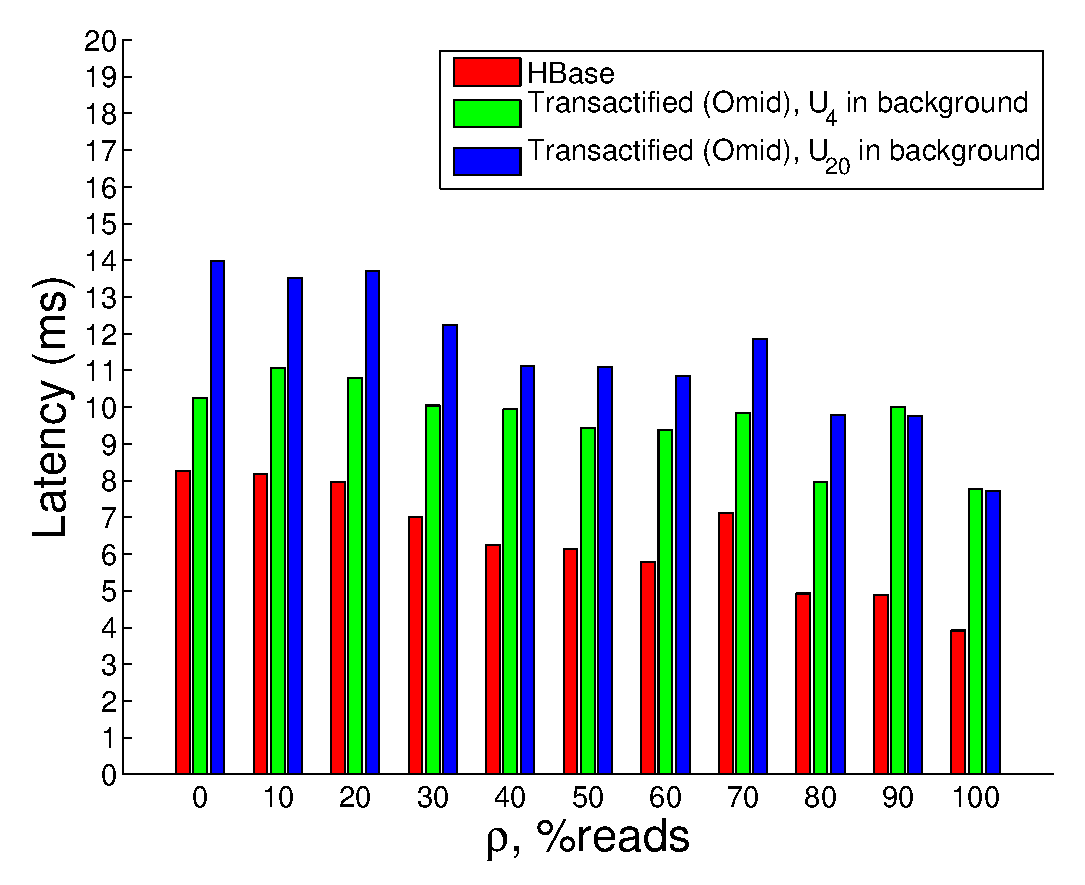
\includegraphics[width=2in]{Figs/matlab/omid_native_latency_u19_10n.eps}}
		\caption{$\uniform{1}$ workload ($\uniform{4}$, $\uniform{20}$ in the background).}
	\end{subfigure}
\quad
  \begin{subfigure}[b]{0.3\textwidth}
		{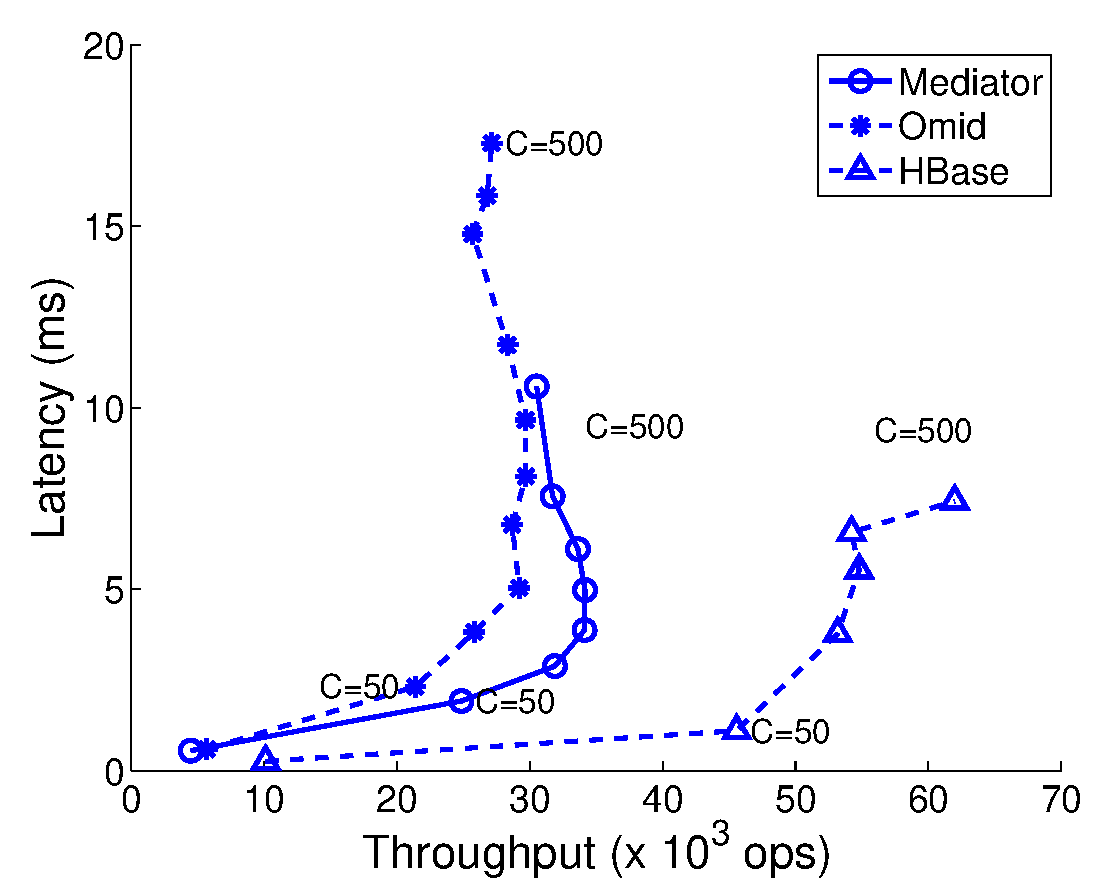
\includegraphics[width=2in]{Figs/matlab/throughput_latency_u1_90r.eps}}
		\caption{Read-dominated $\uniform{1}$ workload.}
  \end{subfigure}%
  \quad
	\begin{subfigure}[b]{0.3\textwidth}
		{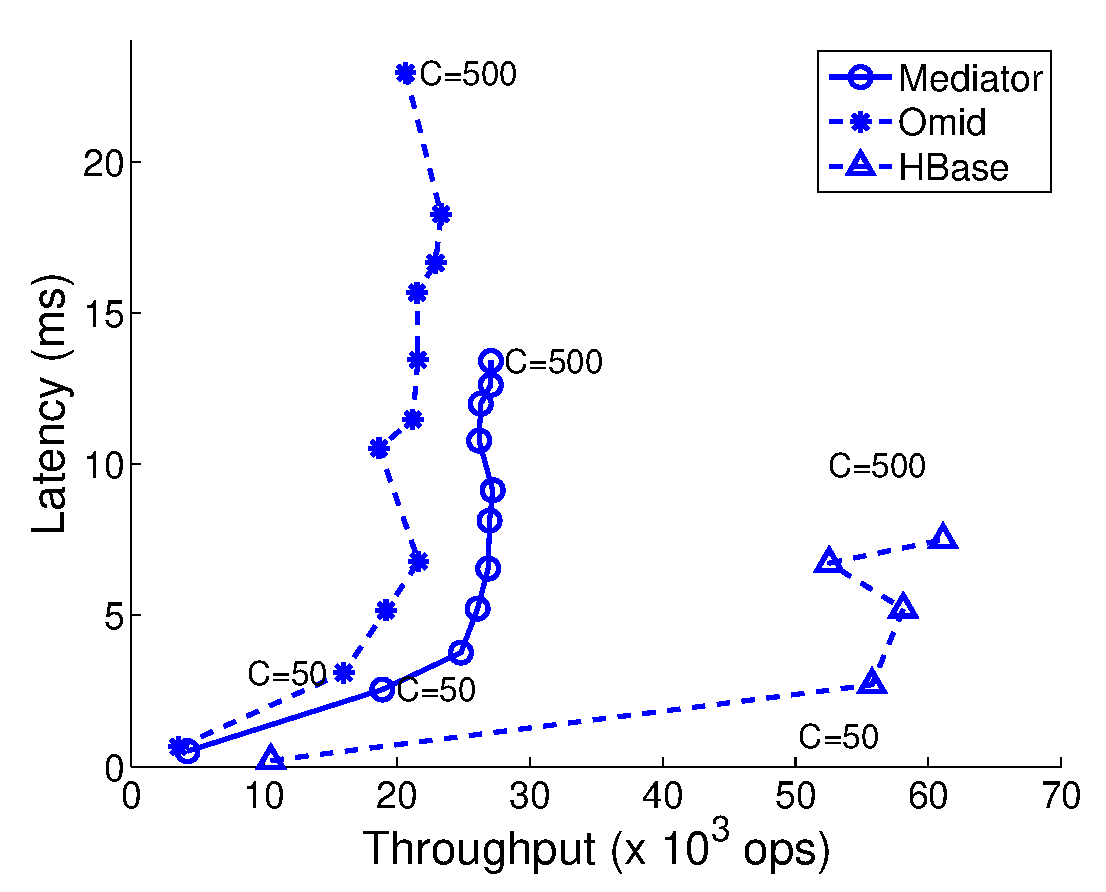
\includegraphics[width=2in]{Figs/matlab/throughput_latency_u1_50r.eps}}
		\caption{Write-intensive $\uniform{1}$ workload.}
	\end{subfigure}
}
\caption{\bf{\small{Transaction processing's performance overhead on gets and puts. 
(a) Latency perspective. HBase compared to Omid's single-operation ($\uniform{1}$) transactions, with larger transactions in the background. 
Fixed number of clients ($C=200$), running read ratio ($0 \leq \rho \leq 1$).
(b,c) Throughput-Latency perspective. HBase compared to Omid's and Mediator's $\uniform{1}$ transactions. 
Running number of clients ($5 \leq C \leq 500$).} }}

\label{fig:txn_only_si}
%\vskip -.2.5in
\end{figure*}

\subsection{Environment}
\label{sec:testing platform}

We utilize a cluster of machines equipped with a $4$-core $2.50$ GHz Xeon(R) L5420 
CPU and $16$ GB RAM. All services are implemented in Java, with the JVM using $4$ GB heap.  
Separate nodes are allocated to the datababse ($10$), the log ($10$),  the TSO ($1$), and the clients ($20$). 

The key-value store is HBase, deployed on top of Hadoop's distributed filesystem, HDFS, with a replication 
factor of $3$. The HBase database (region) servers are co-located with HDFS storage servers (datanodes) for 
efficiency. The dataset under test holds $200$ million records. Each record
is 1 KB long, with a 12 bytes long key. That is, the database's size is
approximately $200$ GB, each server controlling $10\%$ thereof.  The block cache at each server defaults to $40\%$
of the heap.

%In order to explore the settings in which transaction processing introduces a
% meaningful overhead, 
We are interested in latency-oriented applications and therefore focus on
configurations that serve individual operations with low latency.
We address workloads with reasonable locality of gets -- the keys are drawn from
a Zipfian distribution that generates approximately a $90\%$ cache hit rate. The
put latencies are insensitive to key distribution since HBase servers employs
LSM trees~\cite{FDPlus2012} that absorb multiple writes into a memory buffer.
To keep the changes to the database layer minimal, we do not try to optimize the HBase overhead 
by switching off the database's internal write-ahead logging (which is redundant with Mediator's log 
for transactional traffic).
 
We perform a large set of experiments on a variety of workloads. A single experiment performs 
$500{,}000$ gets and puts. Each client node concurrently drives the system's workload through 
up to $40$ concurrent processes of YCSB~\cite{YCSB2010}, a popular load generator. 
The YCSB clients exercise the Mediator, Omid, and HBase API's, depending on the configuration. 

In a single experiment, each YCSB instance drives the same traffic pattern, therefore the cumulative 
workload remains steady over time. In other words, each client generates the same load bandwidth, 
which splits independently among (1) reads and writes, and (2) transactional and native accesses. 
We denote the fraction of reads by $\rho$, and the fraction of native operations by $\nu$. 
In the Omid setting, YCSB transactifies all the original native operations. In both settings, 
transactional accesses are clustered in transactions of varying sizes, picked 
uniformly at random from a range $[1, 2, \ldots, n]$, where $n$ is specified by the 
experiment. We denote this distribution $\uniform{n}$. The larger $n$ is, the wider the spectrum 
of the exercised transaction sizes is -- from a single access to a bulk of operations. 
$\uniform{1}$ is a non-realistic workload (singleton transactions workload is
meaningless) that we use to demonstrate the local-commit optimization. Table~\ref{tab:notation} 
summarizes the notation. 

Mediator log is implemented through Bookkeeper~\cite{Bookkeeper2013}. 
Finally, the TSO employs $1024$-bits-wide Bloom filters.

\setlength{\belowcaptionskip}{0pt}
\setlength{\abovecaptionskip}{6pt}
\begin{table} [t]
\small{
%\hrulefill
\begin{tabular}{lll}
{\bf Notation} & {\bf Description} & {\bf Values} \\
\hline
$C$ & number of concurrent clients & $50, 100, \ldots, 1200$ \\
$\nu$ & ratio of native operations & $0, 0.1, \ldots, 1$ \\
$\rho$ & ratio of get accesses & $0, 0.1, \ldots, 1$  \\
$\uniform{n}$ & transaction size distribution & $\uniform{1}$ (singletons), \\
& (uniform over $[1, 2, \ldots n]$) & $\uniform{4}$, $\uniform{20}$
\end{tabular}
}
%\vskip .1in
\caption{\bf{\small{Workload parameter notation.}}}
\label{tab:notation}
%\vskip -.2.5in
\end{table}

\subsection{Numerical Results -- Snapshot Isolation}
\label{sec:tests:si}

This section studies Mediator's performance under the snapshot isolation consistency model. 

\begin{figure*}
  \centering
  \begin{subfigure}[t]{0.3\textwidth}
   %\flushleft
   \center
		{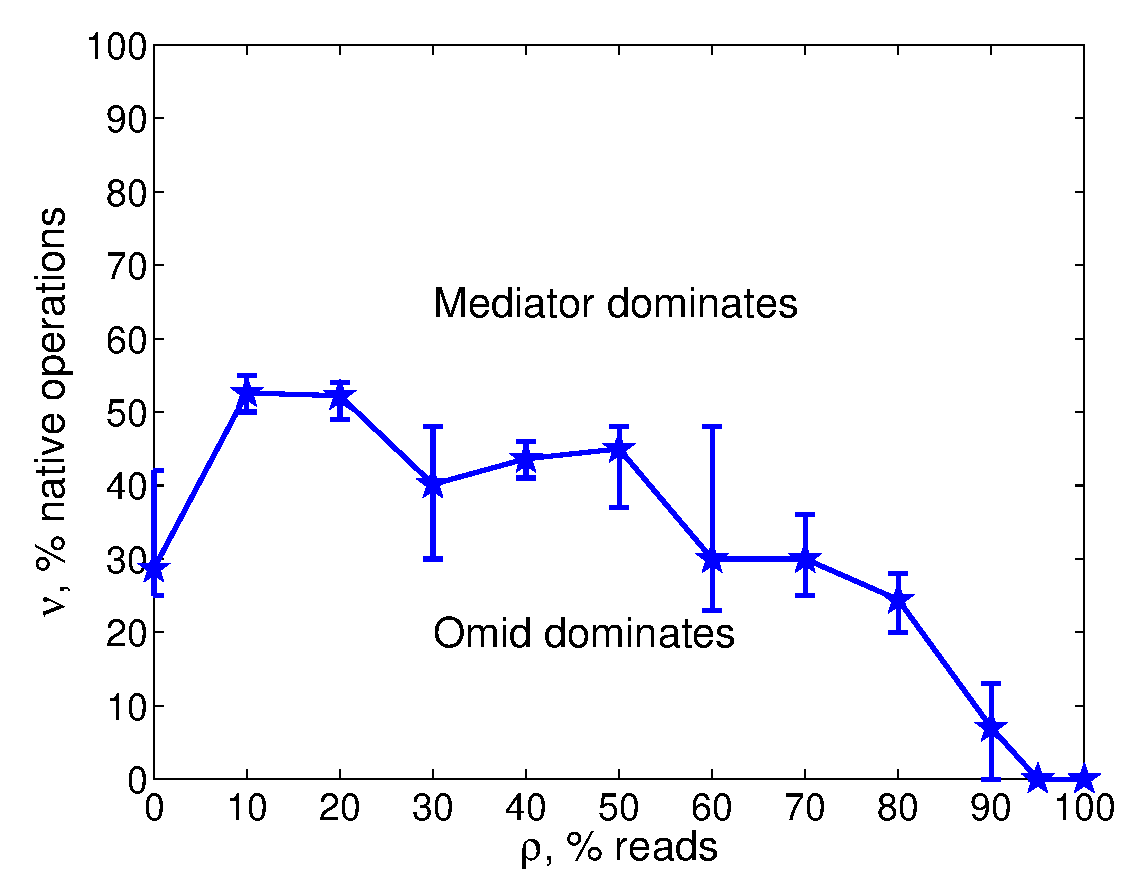
\includegraphics[width=2in]{Figs/matlab/equilibrium_curve_u4.eps}}
		\caption{Equilibrium curve for $\uniform{4}$.}
               \label{fig:heatmap}
  \end{subfigure}%
%\hspace{0.4in}
\quad
	\begin{subfigure}[t]{0.3\textwidth}
		{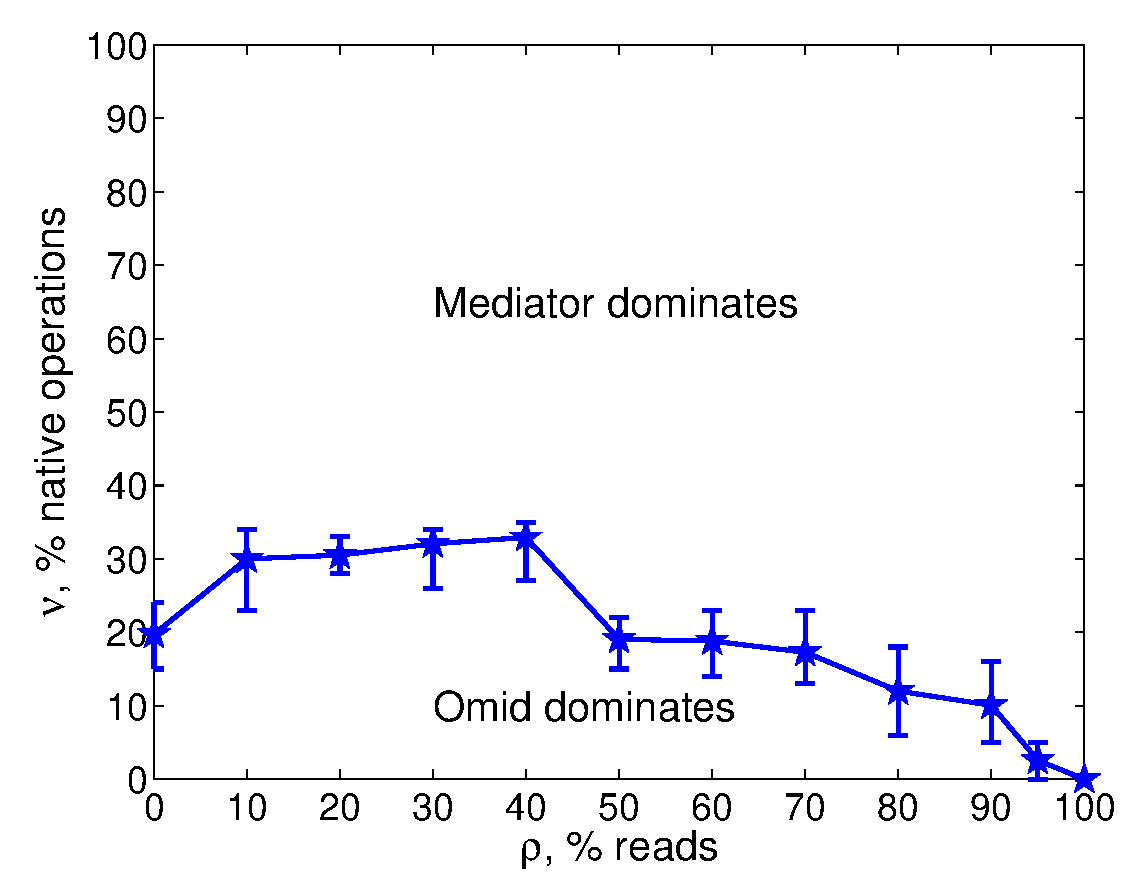
\includegraphics[width=2in]{Figs/matlab/equilibrium_curve_u19.eps}}
		\caption{Equilibrium curve for  $\uniform{20}$.}
       \label{fig:curves}
       \end{subfigure}
\quad
       \begin{subfigure}[t]{0.3\textwidth}
	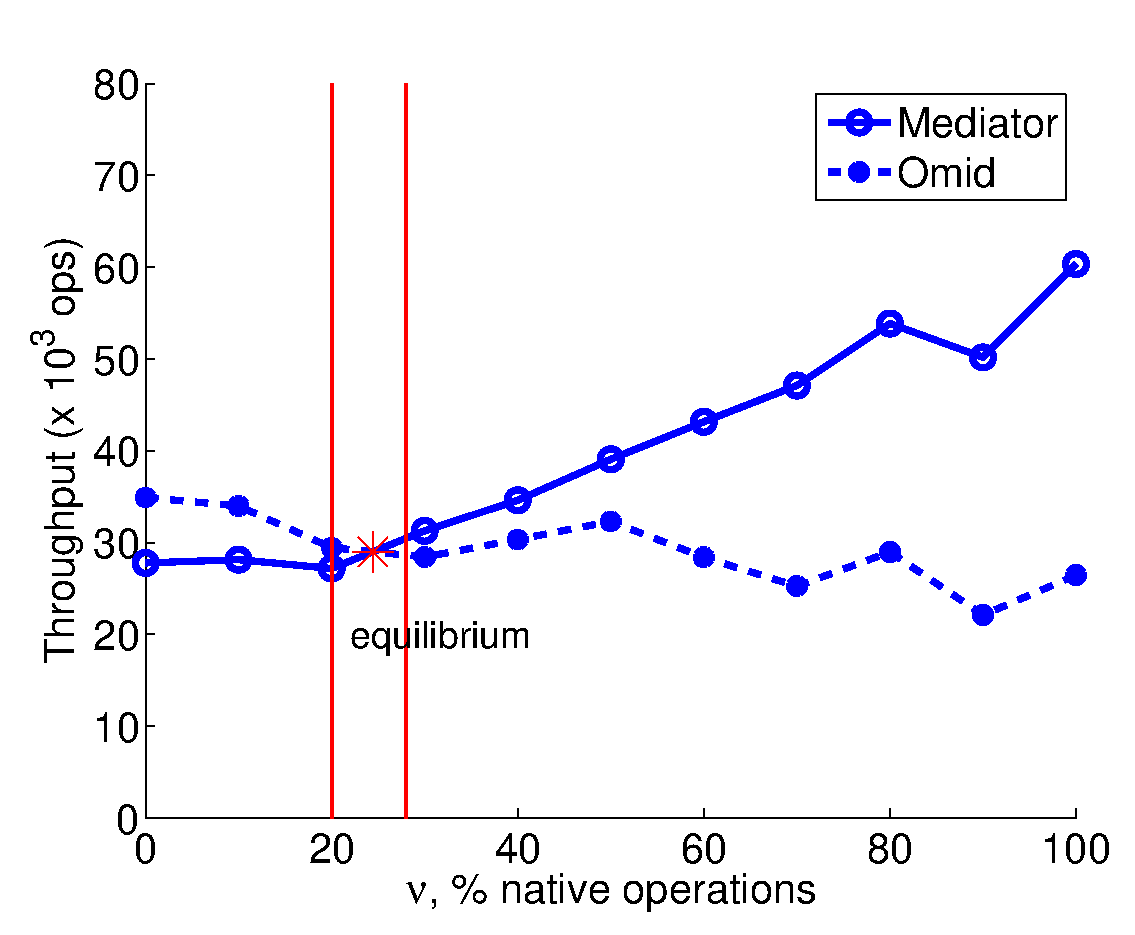
\includegraphics[width=2in]{Figs/matlab/equilibrium_90r_u4.eps}
	\caption{An equilibrium point, $\uniform{4}$, $\rho=0.8$.}
	\end{subfigure}

\caption{\bf{\small{Comfort zones of Mediator and Omid, for a variety of read-write mixes ($0 \leq \rho \leq 1$) 
and transactional-native mixes ($0 \leq \nu \leq 1$). The workload is generated by $200$ clients.
}}}
\label{fig:equilibrium}
\end{figure*}

{\bf Latency Overhead on Single Operations.} 
We start by motivating the advantage of serving native traffic directly. 
Our first experiment demonstrates the surplus to the median latency of native HBase operations 
when the latter are transactified with Omid. We consider three configurations: (1) 100\% native traffic, 
(2) single-operation ($\uniform{1}$) transactions with background $\uniform{4}$ traffic, and 
(3) the same with background $\uniform{20}$ traffic. The workload is driven by 200 clients. 
We explore a variety of read ratios ($0 \leq \rho \leq 1$). 

Figure~\ref{fig:txn_only_si}(a) shows the results. The penalty grows with the fraction of writes
and the background transactions' bulkiness. This is explained as follows. Transactions introduce 
a fixed communication overhead (round trip upon begin and commit), and the TSO state replication 
overhead. The TSO state depends on the number of keys updated by individual transactions, 
i.e., for the same read/write ratio the larger transactions populate a larger state, which translates
to a larger replication overhead, and eventually to larger latencies incurred to short transactions. 
For example, in write-only workloads in which transactified puts run in parallel with $\uniform{20}$ 
transactions, the put latency becomes almost twice as large as that of the native HBase operation.   

The next example provides a different perspective on the same phenomenon. We compare the median
operation latency and the system throughput for the traffic of $100\%$ single operations ($\uniform{1}$), 
in the following scenarios: (1) native operations, (2) the same, transactified with Omid, and (3) the same, 
transactified with Mediator. We observe the performance for varying numbers of clients, and draw the 
throughput-latency curves. All implementations are considered in two settings -- a read-dominated workload 
($\rho=0.9$, Figure~\ref{fig:txn_only_si}(b)), and a write-intensive workload ($\rho=0.5$, Figure~\ref{fig:txn_only_si}(c)). 
We see that even without any bulky transactions in the background, Omid and Mediator are inferior to
bare-metal HBase. For example, Mediator scales to approximately $35$K operations per second (ops) 
in the read-dominated scenario, and to $28$K in the write-intensive one, whereas HBase achieves above 
$55$K ops\footnote{\footnotesize{The same HBase configuration scores much higher throughputs 
for bulk I/O. This setting is not the focus of our experiment.}}. These results emphasize the potential 
of consolidating transactional and non-transactional traffic within the same framework, 
to avoid the overhead of transactifying the latter.

% Face-off!
%\subsubsection{Mixed Traffic} 
%\label{sec:tests:si:mixed}

{\bf Total Throughput.} 
We now turn to our main goal -- contrasting Mediator with Omid on a wide variety of mixed workloads. 
We study the $\uniform{1}$, $\uniform{4}$ and $\uniform{20}$  distributions.   

The $\uniform{1}$ case is an exception -- Mediator is faster than Omid in all configurations
(Figure~\ref{fig:txn_only_si}(b) and Figure~\ref{fig:txn_only_si}(c) demonstrate this for two
specific cases). This happens by the virtue of its no-commit optimization (which
serves single-get transactions) and its local-update optimization (which serves
single-put transactions). Either way, Mediator client does not communicate with
the TSO upon commit skipping consistency checks and logging, hence, the oracle's
state remains void. Upon transaction begin, the state replicated to the client 
is minimal (transaction timestamp), and therefore Mediator's overhead is smaller. Obviously,
if Mediator is faster for all-transactional $\uniform{1}$ traffic, the same holds if part of the workload
is native. 

The comparison becomes interesting for truly mixed workloads, in which native operations
run side by side with transactions of different sizes. Both Omid and Mediator have their strong points.
The former is superior for transactional traffic, since it avoids the WAL overhead (Section~\ref{sec:overview}). 
The latter is faster for native traffic. In this context, the cumulative throughput (in terms of both transactional 
and native operations) is a convenient metric for evaluating the overall system performance. (Note that in 
an environment in which get and put operations are clustered in transactions,
the latency of individual operations is not well-defined.) 

The following experiment employs $200$ clients, and exercises all combinations of read ratios 
($0 \leq \rho \leq 1$) and native access ratios ($0 \leq \nu \leq 1$). In this context, for a given 
read ratio $\rho$, an {\em equilibrium point\/} is the smallest ratio of native operations $\nu$ 
for which Mediator achieves a larger throughput. The collection of equilibrium points for a given 
workload type defines an {\em equilibrium curve}. This curve separates Mediator's and Omid's 
comfort zones. The area above it is the fraction of configurations in which Mediator 
is superior. 

Figure~\ref{fig:equilibrium}(a) and Figure~\ref{fig:equilibrium}(b) portray the equilibrium curves 
for $\uniform{4}$ and $\uniform{20}$, respectively. Every data point is depicted with a $10\%$
confidence interval. Mediator outperforms Omid in a vast majority of configurations -- in particular, 
in any read-write mix with $\nu \geq 50\%$. It is consistently more advantageous for $\uniform{20}$ 
versus $\uniform{4}$, due a better manifestation of write batching in bulk transactions. For both workloads, 
Mediator's dominance is more pronounced for the extreme values of $\rho$. For example, for $\rho=1$, 
the no-commit optimization applies to all transactions, thus reducing the equilibrium point to zero; 
for $\rho=0$, the local-commit optimization applies to singleton transactions
(only part of the workload).

\remove{
Figure~\ref{fig:equilibrium}(b) zooms in on the results from Figure~\ref{fig:equilibrium}(a).
The throughput ratio between Mediator and Omid for the $\uniform{4}$ distribution is depicted 
in a log-scale ``heat map'' presentation. The areas in which Mediator prevails appear in warm 
tones. The zero-isoheight boundary (marked by $\Diamond$) captures the equilibrium curve. 
Note that the absolute performance gaps are bigger in Mediator's dominance area. 
}

Figure~\ref{fig:equilibrium}(c) zooms in on how a single equilibrium point is computed.
For a given read ratio $\rho$, Mediator's throughput monotonically increases with the 
fraction of native traffic $\nu$ (which is natural, since the latter has no overhead). 
On the contrary, Omid's throughput does not grow with $\nu$. This happens because 
the system wraps every individual access as a transaction. For non-singleton 
transactions ($\uniform{4}$ and $\uniform{20}$), the overhead grows disproportionately 
with $\nu$, thus reducing the total throughput. The crossing of the two curves is an equilibrium 
point; the vertical bars mark the areas of statistically significant dominance. 

%\subsubsection{Abort Ratio}
%\label{sec:tests:si:abort_ratio}

{\bf Abort Ratio.} 
We explore the {\em abort ratios\/} incurred by Mediator to user applications --
i.e., the fraction of transactios that get aborted due to (possibly falsely) 	
detected conflicts.  The probability of colliding with concurrent operations grows 
with the fraction of updates and with the transaction size. The 
computation of the write-set intersections is approximate, due to
the use of Bloom filters. Therefore, for write-intensive workloads, 
the fraction of spurious aborts grows as well.  

For short $\uniform{4}$ transactions, the  abort ratios are totally negligible
(below $0.03\%$ under all workloads). For $\uniform{20}$ distribution, the 
ratio remains below $0.1\%$ in most configurations, but hits a high $1.78\%$
in write-intensive settings. This fraction of aborts can be reduced $10$-fold 
by applying wider Bloom filters, but
%, which dramatically decrease the false positive rate. 
this entails a slight performance penalty. %(not presented due to lack of
% space).

\remove{
\begin{figure}[t]
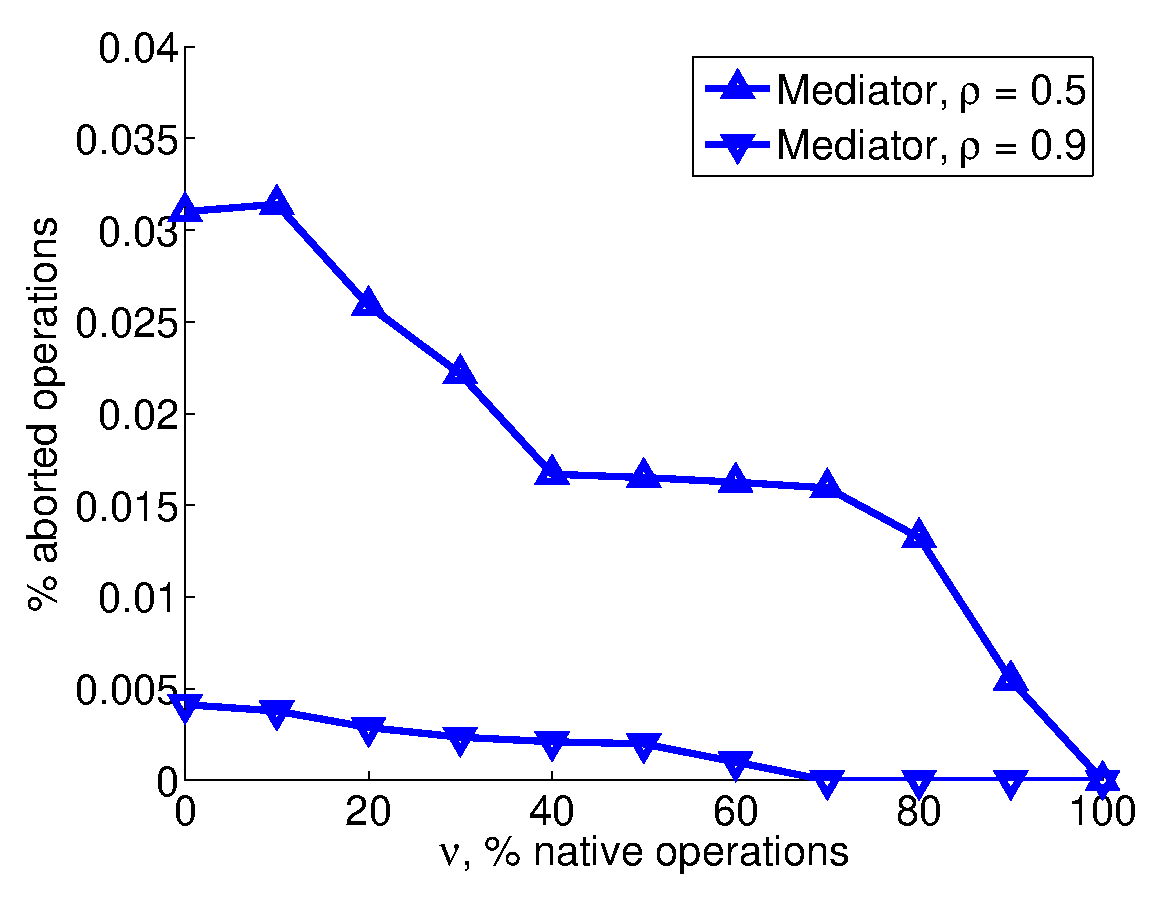
\includegraphics[width=2.5in]{Figs/matlab/abort_ratio_50r_u4.eps}
\caption{\bf{\small{Mediator's abort ratios, for the $\uniform{4}$ workload 
generated by $200$ clients ($0 \leq \nu \leq 1$, $\rho=0.5$ and $\rho=0.9$). 
For read-intensive workloads, the abort ratio is significantly smaller.}}}
\label{fig:abort_ratio}
%\vskip -.2.5in
\end{figure}
}


%\subsubsection{Scalability}
%\label{sec:eval:scalability}

{\bf Scalability.} Finally, we study Mediator's bottlenecks, to get an insight about its 
scalability limits. 
We take a closer look at the $\uniform{4}$ traffic pattern ($\rho=0.5, \nu=0$), 
for the number of clients $C$ ranging from $50$ to $500$. 
Figure~\ref{fig:latency_breakdown} depicts the latency breakdown 
by the time spent on significant internal API's. In this context, the datapath 
calls that happen upon commit (the native conflict check, the WAL, and the database 
write) account for over $70\%$ of transaction latency, whereas TSO's API's consume 
less than $20\%$. For very large numbers of clients, this fraction drops below 
$10\%$, which demonstrates that the TSO scales better than the database. 
The begin timestamp retrieval %$\medserver$.txTimestampRequest() call 
is a non-negligible component. This happens due to the oracle's state replication that 
is piggybacked on this request. 
%($\dbserver$.checkNativeConflicts(), $\logger$.append(), and $\dbserver$.txPut()) 
%($\medserver$.txTimestampRequest() and $\medserver$.txTryCommit()) 

%The database and the logger components are the system's bottlenecks, despite
% the fact that they are both distributed. 
The overhead of write-ahead logging might be reduced 
by employing state-of-the-art shared log services (e.g., Corfu~\cite{Corfu2012} 
uses specialized hardware, and boasts sub-millisecond latencies for loads similar 
to those exercised in our experiment). The potential upside 
of this optimization is approximately $25\%$ reduction of transaction latency.

\begin{figure}
\centering{
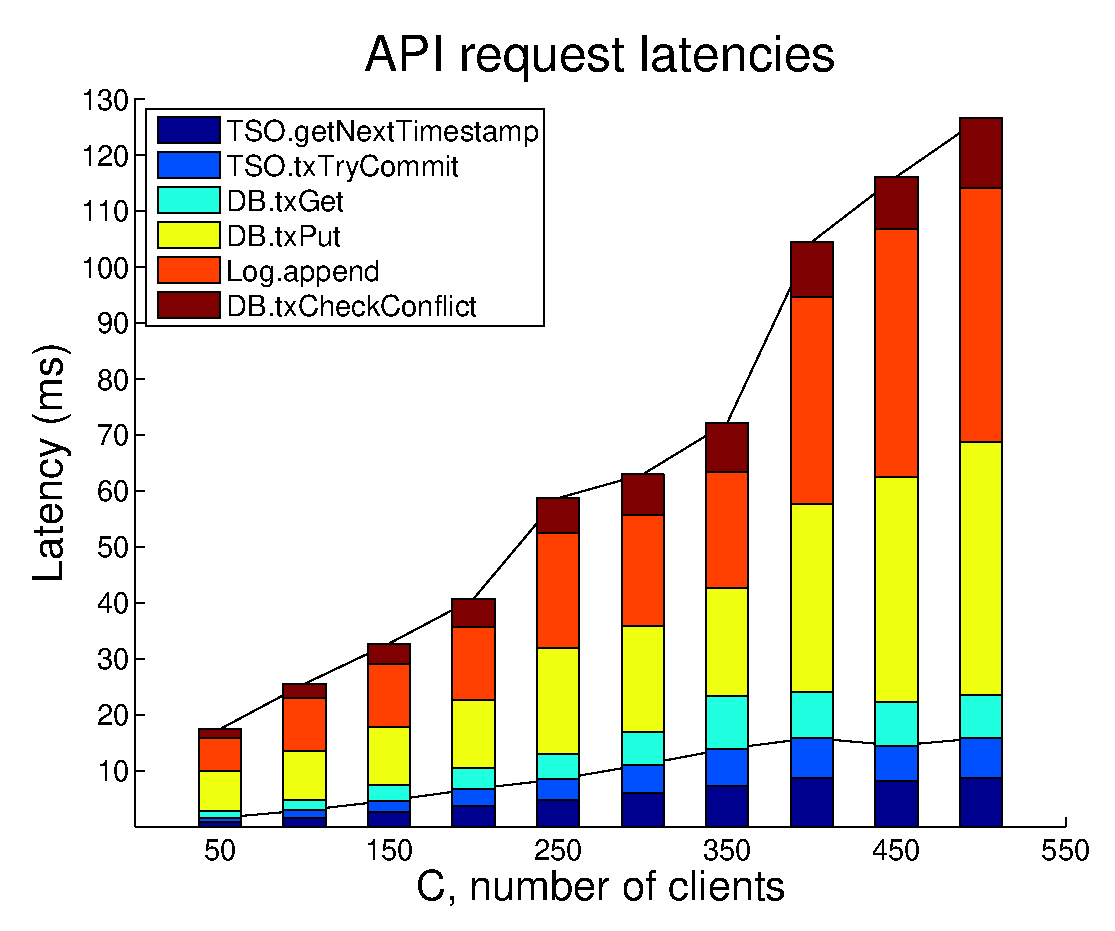
\includegraphics[width=2in]{Figs/matlab/latency_breakdown.eps}
}
\caption{\bf{\small{Breakdown of internal API request latencies, for the $\uniform{4}$ workload 
($\rho=0.5, \nu=0$), with a varying number of clients. The database and the 
logger layers are the execution bottlenecks.}}}
\label{fig:latency_breakdown}
%\vskip -.2.5in
\end{figure}


\subsection{Numerical Results -- Serializability}
\label{sec:tests:ser}

We conclude our experimentation by evaluating the overhead required to support
transaction serializability. In this setting, the algorithm incurs additional 
overhead (sending the transaction's read set to the TSO, in conjunction with the write set), 
and tests for read-write conflicts instead of write-write conflicts (Section~\ref{sec:ser}). 

We compare the serializability implementation's performance with the one for snapshot isolation,
by repeating the experiment in Section~\ref{sec:tests:si}, which evaluates Mediator with transaction-only 
traffic ($\nu=0$). 
%For singleton transactions ($\uniform{1}$), no difference exists, 
%since single-{\em get\/} transactions enjoy the no-commit optimization. 
%The results of comparison for the $\uniform{4}$ transaction size distribution 
%appear in Figure~\ref{fig:ser_comparison}. 
%
For read-dominated workloads ($\rho=0.9$), communication and
processing for serializability support incurs a significant overhead -- up to
$30\%$ less throughput in similar operating points. 
%As explained, this is due to sending all read sets to TSO instead of only 
%the write sets in snapshot isolation. Therefore, the communication and
% processing overheads are increased multiple times. 
%The impact is most pronounced with especially light loads. 
For write-intensive traffic ($\rho=0.5$), the performance gap is negligible. 
These results resonate well with other performance studies in the database 
literature~\cite{Alomari2008,Cahill2008}.


\remove{
\setlength{\abovecaptionskip}{9pt}
\setlength{\belowcaptionskip}{-11pt}
\begin{figure*}
  \centering
  \begin{subfigure}[b]{0.5\textwidth}
		{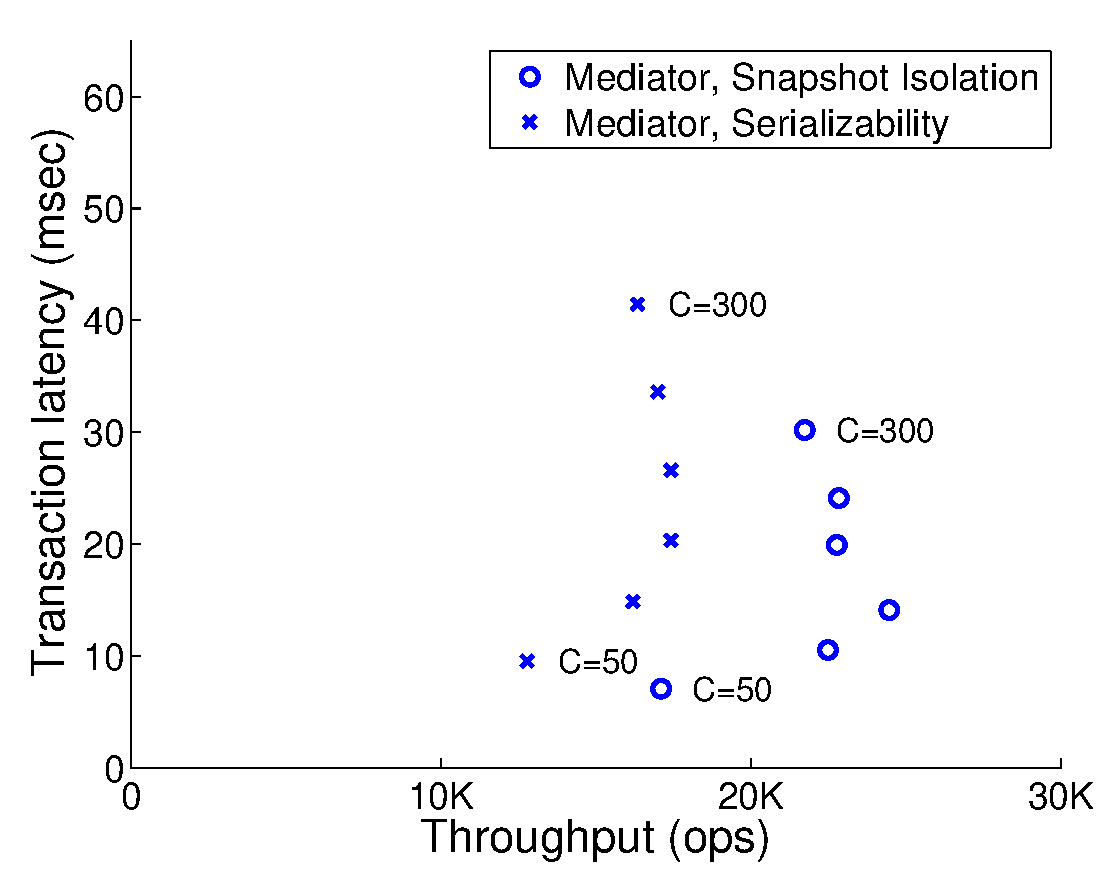
\includegraphics[width=2.5in]{Figs/matlab/throughput_latency_u4_90r_ser.eps}}
		\caption{Read-dominated workload ($\rho=0.9$)}
  \end{subfigure}%
%\hspace{0.4in}
	\begin{subfigure}[b]{0.5\textwidth}
{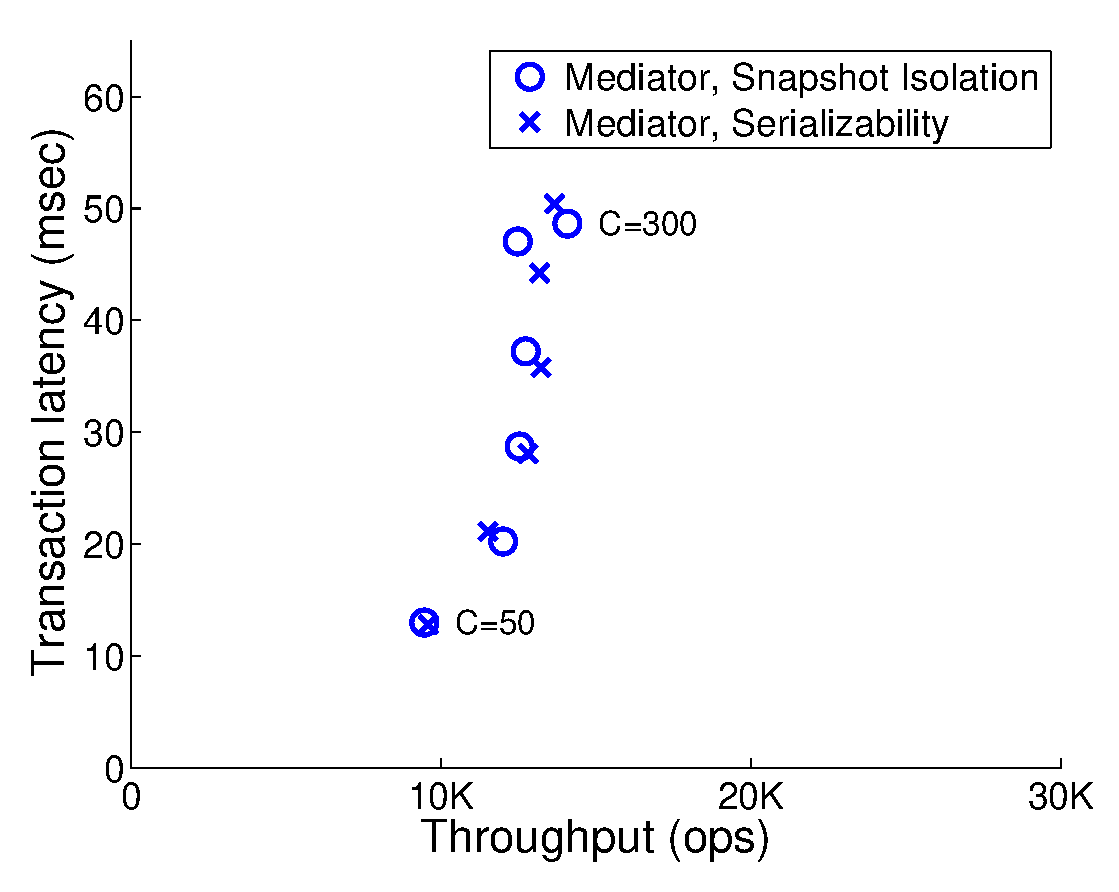
\includegraphics[width=2.5in]{Figs/matlab/throughput_latency_u4_50r_ser.eps}}
		\caption{Write-intensive workload ($\rho=0.5$)}
	\end{subfigure}

\caption{\bf{\small{Evaluation of the performance overhead incurred by supporting the serializability
consistency model. The Mediator implementations of snapshot isolation and serializability are 
compared for the $\uniform{4}$ transaction-only ($\nu=1$) traffic pattern, in the read-dominated 
($\rho=0.9$) and write-intensive ($\rho=0.5$) settings. The performance gap is substantial 
in the first case, and negligible in the second one. }}}
\label{fig:ser_comparison}
%\vskip -.2.5in
\end{figure*}
}
%\hyphenation{su-pports}

\section{Model and Correctness}
\label{sec:correctness}

\remove{
A \emph{database} is a collection of \emph{data items}  uniquely identified by
their keys.
%(in our context, table rows). 
Multiple versions (values) of each item may co-exist 
simultaneously. Each item is a single-writer object, controlled by a 
unique process called {\em data server}. 
%The latter installs  total order among the item's versions. %A data server can atomically write multiple items
%under its control. 

A \emph{transactional processing system} employs \emph{transactions} to execute
pieces of sequential code, namely \emph{operations}, by concurrent asynchrounous
processes. An {implementation} of the system provides routines to execute these
operations. When a process calls a routine we say it \emph{invokes} an
operation, when  the execution of the routine is completed a \emph{response} is
returned.
%A \emph{transaction} is a sequence of operations executed by a single process.
% These include gets and puts on data items, as well as begin, commit and abort operations.
A \emph{begin} operation initializes a transaction and returns 
its handle. A \emph{commit} operation returns an indication whether the transaction 
committed or aborted. An \emph{abort} cancels the transaction and returns an
abort indication.
A \emph{get} operation specifies the key of the data item to read, and returns the value read
by the operation. A \emph{put} operation specifies the key and a value to be
written. Get and put operations return an abort indication if the transaction
in which it is invoked has to abort.
For simplicity of presentation, we do not consider additional operations (e.g., range get queries).
In the rest of the paper we use the terms put/write, and get/read
interchangeably.

After the transaction begins, it executes a sequence of get and put operations, followed by either a commit or an abort. 
\emph{Abort ratio} %of an execution
is the ratio between aborted transactions and transactions that have not invoked the abort operation. 

The collection of data items accessed by a transaction is its data set. 
The data items it puts are its \emph{write set}, and the data items it gets are its 
\emph{read set}. A \emph{read-only} transaction performs only get 
operations (its write set is empty); otherwise, it is an \emph{update}
transaction. A \emph{write-only} transaction is an update transaction with an empty read
set. A \emph{put} transaction is a write-only transaction updating a single
item.

A \emph{native} operation is either a put or a get operation that is not
executed in the context of a transaction. Unlike their transactional
equivalents, native operation never return an abort indication.

%An \emph{implementation} of a transaction processing system provides (1) data
% structures for representing transactions and data items, and (2) algorithms, specified as 
%operations on these data structures. \emph{Asynchronous} processes 
%invoke these operations in order to execute native gets/puts and transactions.
}

We refine the classical definitions of serializability
%~\cite{Papadimitriou1979}
and snapshot isolation (SI) %~\cite{Berenson1995, WeikumTIS2001} 
to apply for mixed traffic executions. Then we outline the safety proofs for our
algorithms.


%We assume native operations are never aborted by the database, and require that
% the transaction processing implementation never aborts them as well.

\subsection{Consistency Models}
\label{sec:models}


A \emph{transactional processing system} employs \emph{transactions} to execute
pieces of sequential code, namely \emph{operations}, by concurrent asynchrounous
processes. An \emph{implementation} of the system provides routines to execute
these operations. When a process calls a routine we say it \emph{invokes} an
operation, when  the execution of the routine is completed a \emph{response} is
returned.

An \emph{execution} is a sequence of invocation and responses of native and
transactional operations starting from the initial configuration of the database. 
%Each operation is assumed to be executed as an atomic step. 
If the last response of a transaction is a commit or abort
indication, then the transaction is \emph{completed}, and is said to be
\emph{committed} or \emph{aborted}, respectively; if a transaction invoked a
commit but not yet received a response then it is \emph{commit-pending};
otherwise, it is \emph{active}. 

In a \emph{serial execution}, native operations and transactions are executed to
completion in isolation one after the other.
\remove{A \emph{committed projection} is attained by 
%keeping all native operations and committed transactions, while 
discarding all active and aborted transactions from the execution.}

A transaction $T$ is \emph{legal} in a % committed projection of a 
serial execution if every read invocation of $x$ in $T$ returns a value that was
written to $x$ in $T$ before the read, or if there are no invocations of write to $x$ in $T$
before the read, then the read returns a value that was last written to $x$
before $T$ by a native put or a committed transaction, or the initial value of
$x$ if no such write to $x$ exists before $T$. A native read $op$ is
\emph{legal} in a % committed projection of a 
serial execution if it returns a value that was last written to $x$
before $op$ by a native put or a committed transaction, or the initial value of
$x$ if no such write to $x$ exists before $op$. A % committed projection of a
serial execution is \emph{legal} if all its committed transactions and native
reads are legal.

%Two executions are \emph{equivalent} if (1)~they consist of the same set of
% transactions and native operations, (2)~both transactional and native gets return the same values in both executions, and 
%(3)~the order of any pair of transactions executed by the same process, as well
%as any pair of read and write operations (native and transactional) accessing
%the same item by the same process is the same in both executions
% (\emph{per-process order}).
An execution $\alpha'$ preserves the \emph{per-process transaction order} of
execution $\alpha$ if it preserves the order of any pair of begin operations executed
by the same process in $\alpha$. An execution $\alpha'$ preserves the
\emph{per-process item order} of execution $\alpha$ if it preserves the order of
any pair of native and transactional operations accessing the
same item and executed by the same process in $\alpha$.

Let $T$ be a committed transaction in an execution $\alpha$. Let $T|read$
($T|write$, $T|all$) be the longest subsequence of $T$ in
$\alpha$ consisting only of $T$'s read (write, read and write, respectively)
invocations and their corresponding responses. 
The transaction $T_r$ is defined as follows: if $T|read$ is empty
then $T_r$ is empty, otherwise $T_r$ is the sequence of a begin invocation and
response appended by $T|read$, a commit invocation and a committed response;
$T_w$ and $T_{rw}$ are defined in a similar way, w.r.t. $T|write$ and
$T|all$.

A \emph{serialization} of an execution $\alpha$ is the sequence
$\sigma_{\alpha}$ that includes a \emph{serialization point} for every native
operation in $\alpha$, $*_{op}$, for every committed transaction, and for
some of the commit-pending transactions in $\alpha$,
$*_{T}$.
The \emph{serial execution} $\alpha'$ corresponding to
$\sigma_{\alpha}$ is defined by replacing each $*_{T}$ with $T_{rw}$ and each
$*_{op}$ with \emph{op}'s invocation and response in
$\alpha$. 


\begin{definition}[serializability] 
An implementation supports \emph{serializability} if any execution $\alpha$ 
has a
serialization, $\sigma_{\alpha}$, such that
the serial execution
$\alpha'$ corresponding to $\sigma_{\alpha}$ is legal and preserves
the per-process transaction order and per-process item order of $\alpha$.
\end{definition}
%$S$ is called the \emph{serialization} of $E$.
%; we assume that this serialization order preserves the per-process order, i.e., transactions of the same process maintain their order.

\remove{
The weaker condition of snapshot isolation 
%was suggested as an efficient alternative to serializability for relational databases. It 
decouples the consistency of the gets and the puts of a transaction.
%into the begin time of the transaction and its commit time, respectively. 
Informally, all reads within a transaction see a consistent view of the
database, as though the transaction operates on a private snapshot of the
database taken before its first read. In addition, concurrent transactions are not allowed to modify the same data.  
%this means each transaction is provided with a snapshot of the database at the time of transaction start. 
\full{For a formal definition, see~\cite[Definition 10.3]{WeikumTIS2001}.}
}
\remove{
A \emph{read point} of a transaction is a sequence of its begin operation
followed by all its get operations. A \emph{write point} of a transaction is a
sequence of its put operations followed by its commit operation.  
In a \emph{snapshot serial execution}, the read points of all transactions, the
write points of all transactions, and all native operations are executed to
completion in isolation one after the other, where each read point precedes its
respective write point.   
The \emph{interval} of a write-only transaction is its commit operation. The
interval of other update transactions starts with the begin operation and ends
with the commit operation of this transaction (if no such commit operation
exists, the interval ends at the end of the execution). 
The interval of a native operation is the operation iteslf.
Two transactions or a transaction and a native operation \emph{overlap} if their
intervals overlap. 
%; otherwise they are non-overlapping.

\begin{definition}[snapshot isolation]
An implementation supports \emph{snapshot isolation} if it satisfies two properties:

\textbf{Snapshot property} A committed projection of any execution is equivalent to some snapshot-serial execution. 
%$S$, such that $S$ satisfies two properties: 

%\noindent
\textbf{Disjoint writes property} The write sets of any pair of overlapping transactions, and any pair of overlapping 
transaction and native put
operation, are disjoint.

%\noindent
%\textbf{Snapshot property} A get, either transactional or native, reading item $r$, returns the last value written to $r$ prior to the transaction's reading point or the native read's, respectively, or the initial value if no such write exists\footnote{At any point in snapshot-serial executions, the last value written to an item is well defined.}.
\end{definition}
}


A \emph{snapshot serialization} of an execution $\alpha$, is the sequence
$\sigma_{\alpha}$ that includes a serialization point for every native
operation in $\alpha$, $*_{op}$, and for every committed transaction and for
some of the commit-pending transactions in $\alpha$ it includes a \emph{read
serialization point} $*_{T_r}$ and a \emph{write serialization point} $*_{T_w}$
such that (i)~$*_{T_r}$ preceeds $*_{T_w}$, (ii)~both $*_{T_r}$ and $*_{T_w}$
are inserted after the invocation of $T$'s begin and before the response of
$T$'s commit in $\alpha$.
The \emph{snapshot serial execution} $\alpha'$ corresponding to
$\sigma_{\alpha}$ is defined by replacing each $*_{T_r}$ with $T_r$ and each
$*_{T_w}$ with $T_w$  and each $*_{op}$ with
\emph{op}'s invocation and response in $\alpha$.

For any execution $\alpha$, consider a snapshot serialization
$\sigma_{\alpha}$ of $\alpha$. The \emph{interval} of a native put
operation \emph{op} is $*_{op}$. The \emph{interval} of a
write-only transactions $T$ is the point $*_{T_w}$. The \emph{interval} of a
read-only transactions $T$ is the point $*_{T_r}$. The \emph{interval} of a
read-write transaction $T$ is the interval between
$*_{T_r}$ and $*_{T_w}$ in $\sigma_{\alpha}$. 
Two transactions or a transaction and a native
put operation \emph{overlap} in $\sigma_{\alpha}$ if their intervals overlap.

\remove{
The \emph{interval} of a write-only transaction is the interval between the
invocation and response of its commit operation.
The \emph{interval} of an update transaction (that is not write-only) is the
interval between the invocation of its begin operation and the response of its commit
operation. If no such response exists, the interval ends at the end of
the execution).
The \emph{interval} of a native operation is the interval between its
invocation and response. Native operations are \emph{atomic}, namely within
their intervals there is no invocation or response of any other operation.
Two transactions or a transaction and a native operation \emph{overlap} if their intervals overlap.
}


\begin{definition}[snapshot isolation]
\remove{
An execution $\alpha$ is \emph{snapshot serializable}, if it has a snapshot
serialization $\sigma_{\alpha}$ such that the serial execution $\alpha'$
corresponding to $\sigma_{\alpha}$ is legal and preserves the per-process item
order in $\alpha$.
}

An implementation supports \emph{snapshot isolation} if any execution $\alpha$ 
%satisfies two properties:
has a snapshot
serialization $\sigma_{\alpha}$ such that:
%\noindent

\textbf{Snapshot property} the snapshot serial execution $\alpha'$
corresponding to $\sigma_{\alpha}$ is legal and preserves the per-process item
order in $\alpha$.
%$\alpha$ is snapshot serializable. 

%\noindent
\textbf{Disjoint writes property} The write sets of any pair of overlapping
transactions, and any pair of overlapping transaction and native put operation
in $\sigma_{\alpha}$, are disjoint.  
\end{definition}

The snapshot property implies that native get operations cannot read an
uncommitted value; for serializability, the same trivially follows from the total order.
The deviation of these definitions from a straightforward extension of classical 
definitions --conceiving native operations as transactions---is twofold:
(1)~native operations cannot abort (while transactions can), 
(2)~similar to traditional NoSQL, both models might flip the order of two
native gets in the serialization (whereas two read transactions by the same
process cannot flip their order). 
For example, a process that sequentially reads two items might observe an older version in the 
second read (e.g., since the items are 
updated in parallel by some transaction).
%In our social application example, when the application displays
%a view covering the status of all the user's friends, it uses native reads
%to access them, and it is ok if one status is not
%up-to-date (as it is being concurrently updated by a transaction).

%\input{safety1} 
\hyphenation{acr-oss}

\section{Related Work}
\label{sec:related}

Transaction processing is a textbook area in database research~\cite{WeikumTIS2001,GrayTP1993}.
It appears in the ANSI SQL standards, 
%\footnote{\footnotesize{\url{http://www.contrib.andrew.cmu.edu/~shadow/sql/sql1992.txt}}}, 
as well as in modern NoSQL technologies that took databases to an unprecedented
scale (e.g.,~\cite{Percolator2010}). The literature defines a wealth of transaction 
consistency models that capture different perceptions of concurrency control 
(e.g.,~\cite{Papadimitriou1979, Berenson1995}). Traditionally, client applications 
sharing a single database instance agree on a single consistency model (or multiple 
levels thereof that subsume each other), and pay the required performance toll. 
%Google's recent paper database~\cite{Spanner2012} claims: {\em we believe it is better 
%to have application programmers deal with performance problems due to overuse of transactions 
%as bottlenecks arise, rather than always coding around the lack of transactions.} 
We posit that this approach is not necessarily required, i.e., it is possible 
to accommodate within the same database two incompatible semantics: 
multi-operation transactional consistency, and atomic read-write consistency
appropriate for simple key-value store applications. 

The database community has been reasoning about transaction semantics since the late 
70's~\cite{Papadimitriou1979}. Serializability %model, which is the most 
%intuitive way to logically serialize a concurrent execution, 
has been widely adopted.
%Two-phase locking is a widely accepted implementation of serializability~\cite{GrayTP1993}. 
The seminal paper by Berenson et al.~\cite{Berenson1995} %discussed the
% advantages and drawbacks of serializability and its different relaxations, and 
introduced the snapshot isolation model. The latter is particularly attractive due to its 
implementations that improve concurrency. 
%
\remove{Fekete et al. laid foundations for making SI executions
serializable~\cite{FeketeTODS2005}.
and authored a series of papers comparing the semantics and performance 
of serializability and snapshot isolation.
%showed that the semantic gap between the two is small, and 
A host of later work~\cite{Cahill2008,Ports2012} suggested practical ways of realizing 
these ideas. Mediator implements both SI and serializability semantics. Its implementation 
is {\em optimistic} -- it lets multiple transactions proceed without interference until commit, 
upon which data conflicts are identified, and some transactions might be aborted~\cite{GrayTP1993}. 
}
\remove{
While that paper focused on restructuring the application code to avoid anomalies, Cahill 
et al.~\cite{Cahill2008} suggested a different approach. Their concurrency control algorithm, 
Serializable Snapshot Isolation, ensures that every execution is serializable, no matter what the 
program does. PostgreSQL was the first database product to adopt this algorithm~\cite{Ports2012}.
}

%Snapshot isolation achieves better overall throughput than serializability, 
%at the expense of aborting some transactions~\cite{Alomari2008, Cahill2008}. 
%We show similar results.  

In databases that support range queries, the literature distinguishes between {\em repeatable
read\/} (RR) and {\em serializability\/} isolation levels, %The former
% guarantees serial execution.The latter 
which subsumes RR, and extends it with a requirement of avoiding {\em phantom
reads\/} (returning two different tuple sets for the same key range to two queries running under the same 
transaction~\cite{GrayTP1993}).  Should Mediator be extended to support
predicate queries, it can use the same transaformation technique
by Fekete et al.~\cite{FeketeTODS2005} to get a phantom-free serializable
implementation.
% phantom freedom through range-sensitive conflict resolution,
%however this is not essential for its core algorithm.
  
Early NoSQL databases, e.g., Google Bigtable~\cite{BigTable2006}, Yahoo! 
PNUTS~\cite{PNUTS2008} and Apache HBase sacrifice strong consistency for extreme 
scalability. Their safety guarantee is single-key atomic reads and writes~\cite{AttiyaDC2004}. 
Google Percolator technology~\cite{Percolator2010} supports multi-operation transactions in Bigtable for incremental maintenance 
of its search index. Percolator
%, which is embedded in Bigtable, 
implements snapshot isolation through database locks. Omid, a transaction 
processor for HBase~\cite{Omid2014}, supports snapshot isolation with a
lock-free protocol. Omid also implements serializability~\cite{OmidEurosys2012}.
%its implementation is external to the database. 
Mediator's design bears similarity with Omid,
however, its algorithm is profoundly different, to capture the new safety properties. 

Google Spanner~\cite{Spanner2012} provides distributed transactions 
across datacenter with a blend of SI (for read-only transactions) and serializability guarantees. 
Spanner implements lock-free read-only transactions and lock-based read-write
transactions. 
%It coordinates locks through a synchronous protocol that can
%tolerate limited discrepancies among physical clocks across multiple locations.
Calvin~\cite{calvin} also addresses globally distributed transactions, albeit in
a different way. It replaces locking with deterministic scheduling that orders
transactions through a global consensus service. 
%Similarly to other transaction processing systems,
SCORe~\cite{Peluso2012} is a serializable partial replication protocol that
guarantees read operations always access a consistent snapshot. It applies a
timestamp management scheme to synchronize the nodes handling the
transaction. Neither one of the above
%Spanner nor Calvin
provide any consistency guarantees to hybrid workloads targeted by Mediator. 
%Investigating how to adapt 
%Mediator to multi-datacenter environments is beyond the scope of our work.

\remove{In a way, Mediator challenges the generic claim in~\cite{Spanner2012}:
``We believe it is better to have application programmers deal with performance problems 
due to overuse of transactions as bottlenecks arise, rather than always coding around 
the lack of transactions.''}

%TM
\emph{Transactional memory} (TM)~\cite{Herlihy2008} is a popular approach for alleviating the difficulty of programming concurrent applications for multi-core and multiprocessing systems. 
TM allows concurrent processes synchronize via in-memory transactions.
\remove{
In practice, TM must allow accessing the same items from inside and outside a transaction; this is crucial both for interoperability with legacy code and for improving the performance of the TM. \emph{Privatization}
mechanisms~\cite{Herlihy2008} allow the programmer to ``isolate'' some items making them private to a process. 
The process can thereafter access them non-transactionally, without interfering with other processes.
}
%RingSTM
Our TSO implementation is inspired by %Spear et al.'s work on 
RingSTM~\cite{Spear2008} -- an %the first TM 
implementation that allows accessing the same items from inside and outside a transaction.
%is inherently livelock-free, while at the same time permitting parallel write-back by concurrent disjoint transactions. 
%In RingSTM, transactions commit by enqueuing an entry onto a global ring,
%and represent their read and write sets by Bloom filters. 
RingSTM is not geared for distributed environments, 
hence our challenges are different.
%thus reducing the overhead of metadata manipulation and inspection. 





\section{Conclusions}
\label{sec:conc}

We presented Mediator -- a transaction processing system
for Web-scale NoSQL databases. Mediator mitigates the consistency 
gaps that arise when transactional and native operations 
are allowed to share the same data in a straightforward way. Mediator 
protects the safety invariants of both API's -- namely, (1) atomic reads 
and writes for the native traffic, and (2) snapshot isolation or serializability
for the transactional traffic. 

Mediator provides weak synchronization between two types of logical clocks: 
the global clock maintained by the transaction processing service, and the 
local clocks of multiple independent database servers. This temporal
fencing mechanism installs a logical order between native
and transactional accesses, despite the fact that the native accesses completely 
bypass Mediator's infrastructure. The protocol is well-founded, and also 
extremely lightweight compared to physical clock synchronization.

Mediator preserves the original performance of native traffic, while incurring minor impact on transactional operations. A large-scale evaluation 
shows that this design choice strikes a favorable tradeoff. Namely, it demonstrates
that performance-wise, Mediator's approach is superior to automatic transactification 
of native operations, for a vast majority of our tested workloads. We also
show that spurious aborts -- the price paid for preserving 
the best of both worlds -- are very infrequent. 
%which introduces a considerable overhead, 








%ACKNOWLEDGMENTS are optional
\section{Acknowledgments}
We thank Daniel Gomez-Ferro for his relentless help with 
explaining Omid's design. We thank Flavio Junqueira, 
Ronny Lempel and Mark Shovman for stimulating discussions.

%
% The following two commands are all you need in the
% initial runs of your .tex file to
% produce the bibliography for the citations in your paper.
\bibliographystyle{abbrv}
\bibliography{mediator}  % sigproc.bib is the name of the Bibliography in this
% case You must have a proper ".bib" file
%  and remember to run:
% latex bibtex latex latex
% to resolve all references
%
% ACM needs 'a single self-contained file'!
%
%APPENDICES are optional
%\balancecolumns
%\renewcommand{\full}[1]{#1}
%\renewcommand{\short}[1]{}
%\appendix

\end{document}
